% -*- TeX-engine: luatex -*-
\documentclass[presentation,aspectratio=43, 10pt]{beamer}
\setbeamersize{text margin left=0.5cm, text margin right=0.5cm}
\usepackage{pifont}
\newcommand{\cmark}{\ding{51}}
\newcommand{\xmark}{\ding{55}}
\usepackage{standalone}
\usepackage{svg}
\usepackage{booktabs}
\titlegraphic{
\includegraphics[height=1.25cm]{firedrake-word}\hfill
\includegraphics[height=1.25cm]{durham-logo}}
\usepackage{appendixnumberbeamer}
\usepackage{amsmath}
\usepackage{amssymb}
\usepackage{mathtools}
\usepackage{hyperref}
\usepackage{xspace}
\newcommand{\arxivlink}[2]{{\texttt{arXiv:\,\href{https://arxiv.org/abs/#1}{#1\,[#2]}}}}

\newcommand{\honev}{\ensuremath{{H}^1(\Omega; \mathbb{R}^d)}\xspace}
\newcommand{\ltwov}{\ensuremath{{L}^2(\Omega; \mathbb{R}^d)}\xspace}
\newcommand{\ltwo}{\ensuremath{{L}^2(\Omega)}\xspace}
\newcommand{\inner}[1]{\left\langle #1 \right \rangle}
\usepackage[lined,commentsnumbered]{algorithm2e}

\let\star\relax
\DeclareMathOperator{\star}{star}
\DeclareMathOperator{\closure}{closure}
\usepackage{minted}
\usepackage[url=false,
doi=true,
isbn=false,
style=authoryear,
maxnames=5,
giveninits=true,
uniquename=init,
bibencoding=utf8,
backend=biber]{biblatex}
\renewcommand{\bibfont}{\fontsize{7}{7}\selectfont}
\addbibresource{references.bib}
\setbeamertemplate{bibliography item}[triangle]
\defbibenvironment{bibliography}
  {\list{}
     {\settowidth{\labelwidth}{\usebeamertemplate{bibliography item}}%
      \setlength{\leftmargin}{\labelwidth}%
      \setlength{\rightmargin}{\labelwidth}%
      \setlength{\labelsep}{\biblabelsep}%
      \addtolength{\leftmargin}{\labelsep}%
      \setlength{\itemsep}{\bibitemsep}%
      \setlength{\parsep}{\bibparsep}}}
  {\endlist}
  {\item}

\setlength{\bibitemsep}{0.5ex}
\setlength{\fboxsep}{1pt}

\renewbibmacro{in:}{}
\DeclareFieldFormat[article]{volume}{\textbf{#1}}
\DeclareFieldFormat{doi}{%
  doi\addcolon%
  {\scriptsize\ifhyperref{\href{http://dx.doi.org/#1}{\nolinkurl{#1}}}
    {\nolinkurl{#1}}}}
\AtEveryBibitem{%
\clearfield{pages}%
\clearfield{issue}%
\clearfield{number}%
}

\DeclareMathOperator{\grad}{grad}
\let\div\relax
\DeclareMathOperator{\div}{div}
\DeclareMathOperator{\curl}{curl}
\DeclareMathOperator{\range}{range}
\DeclareMathOperator{\sym}{sym}
\usetheme{metropolis}
\setbeamertemplate{title graphic}{
  \vbox to 0pt {
    \vspace*{1em}
    \inserttitlegraphic%
  }%
  \nointerlineskip%
}
\metroset{background=light,progressbar=frametitle,numbering=counter,block=fill}

% https://www.dur.ac.uk/marketingandcommunications/marketing/branding/colourpalette/
% Most of these are indistinguishable to those suffering colour blindness
\definecolor{purple}{HTML}{68246D}
\definecolor{blue}{HTML}{002A41}
\definecolor{red}{HTML}{BE1E2D}
\definecolor{cyan}{HTML}{00AEEF}
\definecolor{yellow}{HTML}{FFD53A}
\definecolor{green}{HTML}{00D53A}

\newenvironment{variableblock}[3]
{\setbeamercolor{block body}{#2}
\setbeamercolor{block title}{#3}
\begin{block}{#1}}%
{\end{block}}
  
\newenvironment{challenge}[1]%
{\begin{variableblock}{#1}{bg=red!20,fg=black}{bg=red,fg=white}}%
{\end{variableblock}}

\newenvironment{answer}[1]%
{\begin{variableblock}{#1}{bg=cyan!20,fg=black}{bg=cyan,fg=white}}%
{\end{variableblock}}

\renewenvironment{exampleblock}[1]%
{\begin{variableblock}{#1}{bg=green!20,fg=black}{bg=green,fg=white}}%
{\end{variableblock}}

\setbeamercolor{normal text}{
  fg=blue,
  bg=white
}
\setbeamercolor{alerted text}{
  fg=red
}
\setbeamercolor{example text}{
  fg=blue
}

\setbeamercolor{palette primary}{%
  use=normal text,
  fg=normal text.bg,
  bg=purple,
}

\usetheme{metropolis}

\author{Lawrence Mitchell\inst{1,*} \\
  \and {\scriptsize
    P.~E.~Farrell (Oxford)
    \and
    M.~G.~Knepley (Buffalo)
    \and
    F.~Wechsung (Oxford)}}
\institute{
  \inst{1}Department of Computer Science, Durham University\\
  \inst{*}\texttt{lawrence.mitchell@durham.ac.uk}}

\date{February 12, 2020}
\title{PCPATCH: topological construction of multigrid relaxation methods}

\usepackage{tikz}
\usetikzlibrary{trees,calc,positioning}
\usetikzlibrary{shapes, shapes.geometric,decorations.pathreplacing}
\usetikzlibrary{arrows,arrows.meta,chains,positioning,fit,backgrounds,calc,shapes,
  shadows,scopes,decorations.markings,plotmarks}

\newcommand*{\tettextsize}{\footnotesize}
\tikzstyle{line} = [draw, -, thick]
\tikzstyle{nodraw} = [draw, fill, circle, minimum width=0pt, inner sep=0pt]
\tikzstyle{sieve} = [line, circle, font=\tettextsize, inner sep=0pt,
  minimum size=12pt]

\tikzstyle{cell} = [sieve, fill=blue!60]
\tikzstyle{facet} = [sieve, fill=green!35]
\tikzstyle{edge} = [sieve, fill=red!35]
\tikzstyle{vertex} = [sieve, fill=blue!35]

% https://tex.stackexchange.com/questions/27171/padded-boundary-of-convex-hull
\newcommand{\convexpath}[2]{
  [
  create hullcoords/.code={
    \global\edef\namelist{#1}
    \foreach [count=\counter] \nodename in \namelist {
      \global\edef\numberofnodes{\counter}
      \coordinate (hullcoord\counter) at (\nodename);
    }
    \coordinate (hullcoord0) at (hullcoord\numberofnodes);
    \pgfmathtruncatemacro\lastnumber{\numberofnodes+1}
    \coordinate (hullcoord\lastnumber) at (hullcoord1);
  },
  create hullcoords
  ]
  ($(hullcoord1)!#2!-90:(hullcoord0)$)
  \foreach [
  evaluate=\currentnode as \previousnode using \currentnode-1,
  evaluate=\currentnode as \nextnode using \currentnode+1
  ] \currentnode in {1,...,\numberofnodes} {
    let \p1 = ($(hullcoord\currentnode) - (hullcoord\previousnode)$),
    \n1 = {atan2(\y1,\x1) + 90},
    \p2 = ($(hullcoord\nextnode) - (hullcoord\currentnode)$),
    \n2 = {atan2(\y2,\x2) + 90},
    \n{delta} = {Mod(\n2-\n1,360) - 360}
    in
    {arc [start angle=\n1, delta angle=\n{delta}, radius=#2]}
    -- ($(hullcoord\nextnode)!#2!-90:(hullcoord\currentnode)$)
  }
}

\graphicspath{{./\jobname.figures/}{../pictures/}}

\usepackage{cleveref}
\begin{document}

\maketitle

\begin{frame}[t]
  \frametitle{Some motivating schemes}
  \begin{onlyenv}<1>
    \begin{block}{Coupled multigrid for Stokes/Navier--Stokes}
      \emph{In the SCGS scheme four velocites and one pressure
      corresponding to one finite difference node are simultaneously
      updated by inverting a (small) matrix of equations.}

      \begin{center}
        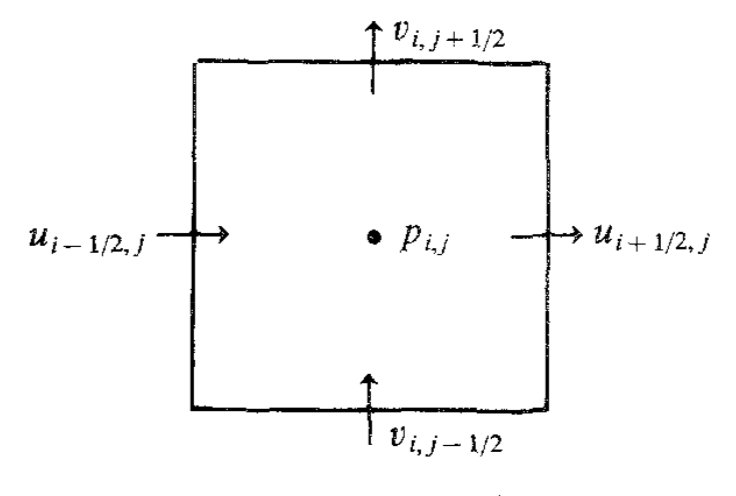
\includegraphics[height=3cm]{vanka}
      \end{center}
      {\hfill \textcite{Vanka:1986}}
    \end{block}
  \end{onlyenv}
  \begin{onlyenv}<2>
    \begin{block}{$p$-independent preconditioners for elliptic problems}
      \emph{[Each subspace is generated from]
      $V_i^p = V^p \cap H^1_0(\Omega_i^{'})$ where $\Omega_i^{'}$ is the open square
      centered at the ith vertex}
      \begin{center}
        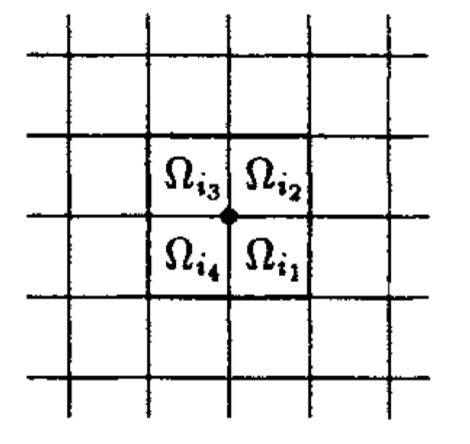
\includegraphics[width=3cm]{pavarino}
      \end{center}
      {\hfill \textcite{Pavarino:1993}}
    \end{block}
  \end{onlyenv}

  \begin{onlyenv}<3>
    \begin{block}{Multigrid for nearly incompressible elasticity}
      \emph{The suggested smoother is a block Jacobi smoother, which takes
      care of the kernel [\dots]. These kernel basis functions are
      captured by subspaces $V_{l,i}$ as shown}
      \begin{center}
        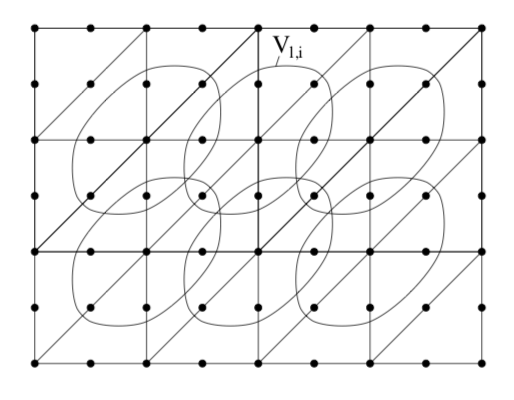
\includegraphics[height=3.25cm]{schoeberl}
      \end{center}
      {\hfill\textcite{Schoeberl:1999}}
    \end{block}
  \end{onlyenv}

  \begin{onlyenv}<4>
    \begin{block}{Multigrid in $H(\div)$ and $H(\curl)$}
      \emph{To define the Schwarz smoothers, we can use a decomposition of
      $V_h$ into local patches consisting of all elements surrounding
      either an edge or a vertex.}

      \begin{center}
        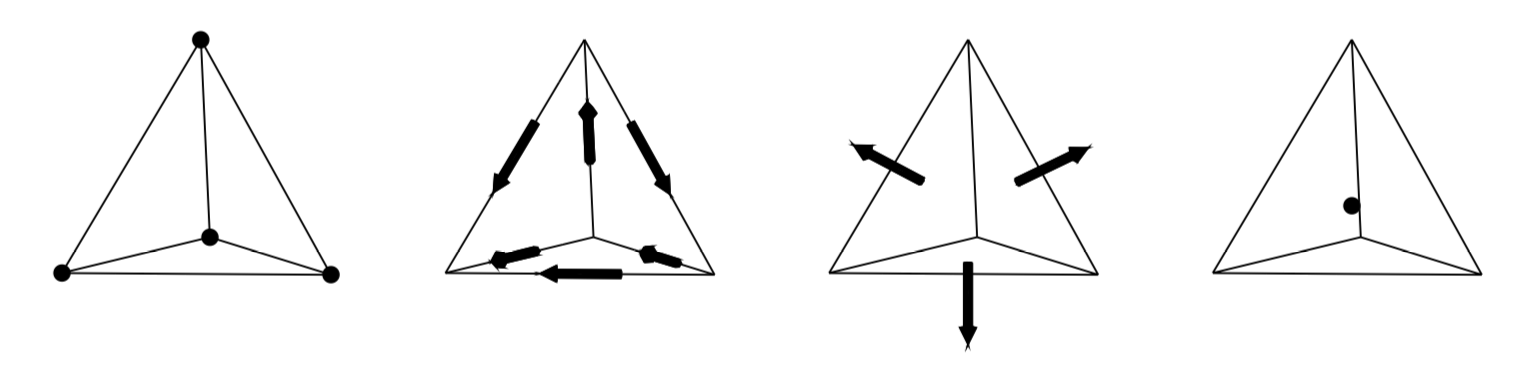
\includegraphics[height=2.5cm]{arnold}
      \end{center}
      {\hfill\textcite{Arnold:2000}}
    \end{block}
  \end{onlyenv}

  \begin{onlyenv}<5>
    \begin{block}{An augmented Lagrangian approach to the Oseen problem}
      \emph{We use a block Gauss-Seidel method [\dots] based on the
      decomposition $V_h = \sum_{i=0}^l V_i$. [\dots For] P2-P0 finite
      elements the natural choice is to gather nodel DOFs for velocity
      inside ovals [around a vertex]}

      \begin{center}
        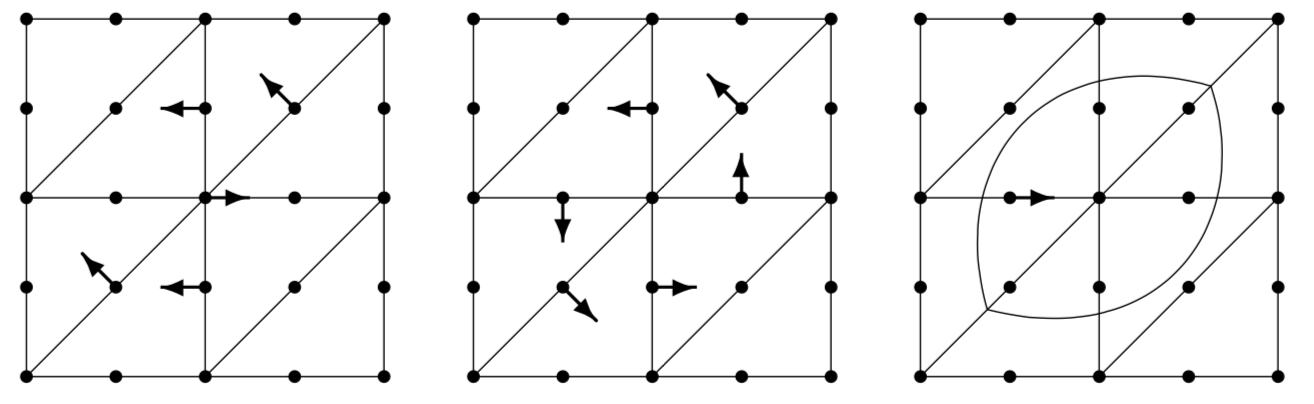
\includegraphics[height=2.5cm]{benzi}
      \end{center}
      {\hfill \textcite{Benzi:2006}}
    \end{block}
  \end{onlyenv}
  \begin{onlyenv}<6>
    \begin{block}{Multigrid for nearly incompressible elasticity}
      \emph{The advantageous consequence of this result is that the
        macro star gives a kernel-capturing space decomposition with
        small support, suitable for use as a multigrid relaxation
        method.}
      \begin{center}
        \begin{tikzpicture}[scale=1.5,
          dof/.style={blue, postaction={decorate,decoration={markings,
          mark=at position 0.5 with {\draw[solid, fill=blue, blue] circle (0.08);}}}
          }]
          \coordinate (0-0) at (1.5, 0);
          \coordinate (0-1) at (3, 0);
          \coordinate (1-0) at ($(0-0) + (120:1.5)$);
          \coordinate (1-1) at ($(1-0) + (1.5, 0)$);
          \coordinate (1-2) at ($(1-0) + (3, 0)$);
          \coordinate (2-0) at ($(1-0) + (60:1.5)$);
          \coordinate (2-1) at ($(2-0) + (1.5, 0)$);
          \foreach \i in {0, 1, 2} {
          \foreach \j in {0, 1} {
          \draw[fill=blue, blue] (\i-\j) circle (0.053333);
          }
          }
          \draw[fill=blue, blue] (1-2) circle (0.053333);

          \coordinate (bc0) at (barycentric cs:0-0=1,1-0=1,1-1=1);
          \coordinate (bc1) at (barycentric cs:0-0=1,0-1=1,1-1=1);
          \coordinate (bc2) at (barycentric cs:0-1=1,1-1=1,1-2=1);
          \coordinate (bc3) at (barycentric cs:1-0=1,1-1=1,2-0=1);
          \coordinate (bc4) at (barycentric cs:1-1=1,2-0=1,2-1=1);
          \coordinate (bc5) at (barycentric cs:1-1=1,2-1=1,1-2=1);
          \foreach \i in {0, 1, 2, 3, 4, 5} {
          \draw[fill=blue, blue] (bc\i) circle (0.053333);
          }

          \draw[dof, line join=miter, thick] (0-0) -- (0-1);
          \draw[dof, line join=miter, thick] (0-1) -- (1-2);
          \draw[dof, line join=miter, thick] (1-2) -- (2-1);
          \draw[dof, line join=miter, thick] (2-1) -- (2-0);
          \draw[dof, line join=miter, thick] (2-0) -- (1-0);
          \draw[dof, line join=miter, thick] (1-0) -- (0-0);

          \draw[dof, line join=miter, thick] (0-0) -- (1-1);
          \draw[dof, line join=miter, thick] (0-1) -- (1-1);
          \draw[dof, line join=miter, thick] (1-0) -- (1-1);
          \draw[dof, line join=miter, thick] (1-2) -- (1-1);
          \draw[dof, line join=miter, thick] (2-0) -- (1-1);
          \draw[dof, line join=miter, thick] (2-1) -- (1-1);

          \draw[dof, line join=miter, thick] (0-0) -- (bc0);
          \draw[dof, line join=miter, thick] (1-0) -- (bc0);
          \draw[dof, line join=miter, thick] (1-1) -- (bc0);

          \draw[dof, line join=miter, thick] (0-0) -- (bc1);
          \draw[dof, line join=miter, thick] (0-1) -- (bc1);
          \draw[dof, line join=miter, thick] (1-1) -- (bc1);

          \draw[dof, line join=miter, thick] (0-1) -- (bc2);
          \draw[dof, line join=miter, thick] (1-2) -- (bc2);
          \draw[dof, line join=miter, thick] (1-1) -- (bc2);

          \draw[dof, line join=miter, thick] (2-0) -- (bc3);
          \draw[dof, line join=miter, thick] (1-0) -- (bc3);
          \draw[dof, line join=miter, thick] (1-1) -- (bc3);

          \draw[dof, line join=miter, thick] (2-1) -- (bc4);
          \draw[dof, line join=miter, thick] (2-0) -- (bc4);
          \draw[dof, line join=miter, thick] (1-1) -- (bc4);

          \draw[dof, line join=miter, thick] (1-2) -- (bc5);
          \draw[dof, line join=miter, thick] (2-1) -- (bc5);
          \draw[dof, line join=miter, thick] (1-1) -- (bc5);
          \begin{scope}[on background layer]
            \draw[cyan, fill=cyan] ([shift={(60:5pt)}]0-0) --
            ([shift={(120:5pt)}]0-1) --
            ([shift={(180:5pt)}]1-2) --
            ([shift={(240:5pt)}]2-1) --
            ([shift={(300:5pt)}]2-0) --
            ([shift={(0:5pt)}]1-0) --
            cycle;
          \end{scope}
        \end{tikzpicture}
      \end{center}
      {\hfill\textcite{Farrell:2020}}
    \end{block}
  \end{onlyenv}
  \begin{onlyenv}<7>
    \begin{block}{Augmented Lagrangian for 3D Navier--Stokes}
      \begin{center}
        \begin{tikzpicture}[scale=0.55,
          every node/.style={scale=0.55, draw=black, thick, anchor=west},
          grow via three points={one child at (0.0,-0.7) and
            two children at (0.0,-0.7) and (0.0,-1.4)},
          edge from parent path={(\tikzparentnode.210) |- (\tikzchildnode.west)}]
          \node {Continuation}
          child { node {Newton solver with line search}
            child { node {Krylov solver (FGMRES)}
              child { node {Block preconditioner}
                child { node {Approximate Schur complement inverse}}
                child { node {F-cycle on augmented momentum block}
                  child { node {Coarse grid solver}
                    child { node {LU factorization}}
                  }
                  child [missing] {}
                  child { node {Prolongation operator}
                    child { node[fill=cyan, draw=cyan!50!black] {Local solves over coarse cells}}
                  }
                  child [missing] {}
                  child { node {Relaxation}
                    child { node {GMRES}
                      child { node[fill=cyan, draw=cyan!50!black] {Additive star iteration}}
                    }
                  }
                }
              }
            }
          };
        \end{tikzpicture}
      \end{center}
      {\hfill \textcite{Farrell:2019}}
    \end{block}
  \end{onlyenv}
\end{frame}

\begin{frame}[t]
  \frametitle{Parallel subspace corrections \parencite{Xu:1992}}
  Find $u \in V$ such that
  \begin{equation*}
    a(u, v) = (f, v) \text{ for all } v \in V.
  \end{equation*}
  \begin{algorithm}[H]
    \SetKwInOut{Input}{input}\SetKwInOut{Output}{output}
    \Input{Space decomposition $V = \sum_{i=1}^J V_i$}
    \Input{Initial guess $u_k \in V$}
    \Input{Weighting operators $w_i : V_i \to V_i$}
    \Output{Updated guess $u_{k+1} \in V$}
    \BlankLine
    \For{$i = 1$ \KwTo $J$}{
      Find $\delta u_i \in V_i$ such that
      \begin{equation*}
        \begin{aligned}
          a(\delta u_i, v_i) &= (f, v_i) - a(u_k, v_i) && \text{ for
            all } v_i \in V_i. && \text{ linear case}\\
          F(u_k + \delta u_i; v_i) &= 0 && \text{ for all } v_i \in
          V_i. && \text{ nonlinear case}
        \end{aligned}
      \end{equation*}
    }
    $u_{k+1} \gets u_k + \sum_{i=1}^{J} w_i(\delta u_i)$
  \end{algorithm}
\end{frame}

\begin{frame}[t]
  \frametitle{Sequential subspace corrections \parencite{Xu:1992}}
  Find $u \in V$ such that
  \begin{equation*}
    a(u, v) = (f, v) \text{ for all } v \in V.
  \end{equation*}
\begin{algorithm}[H]
  \SetKwInOut{Input}{input}\SetKwInOut{Output}{output}
  \Input{Space decomposition $V = \sum_{i=1}^J V_i$}
  \Input{Initial guess $u_k \in V$}
  \Output{Updated guess $u_{k+1} \in V$}
  \BlankLine
  \For{$i = 1$ \KwTo $J$}{
    Find $\delta u_i \in V_i$ such that
    \begin{equation*}
        \begin{aligned}
          a(\delta u_i, v_i) = (f, v_i) - a(u_{k + (i-1)/J}, v_i) && \text{ for
            all } v_i \in V_i. && \text{ linear case}\\
          F(u_{k + (i-1)/J} + \delta u_i; v_i) = 0 && \text{ for all } v_i \in
          V_i. && \text{ nonlinear case}
        \end{aligned}
    \end{equation*}
    $u_{k+i/J} \gets u_{k + (i-1)/J} + \delta u_i$
  }
\end{algorithm}
\end{frame}

\begin{frame}
  \frametitle{Example space decompositions}
  \begin{exampleblock}{Jacobi or Gau\ss-Seidel}
    \vspace{0.5\baselineskip}
    \begin{columns}
      \begin{column}{0.5\textwidth}
        \begin{equation*}
          V = \sum_{i=1}^{N} \operatorname{span} \{\phi_i\}
        \end{equation*}
      \end{column}
      \begin{column}{0.5\textwidth}
        $\{\phi_1, \dots, \phi_N\}$ a basis for $V$.
      \end{column}
    \end{columns}
  \end{exampleblock}
  \begin{exampleblock}{Domain decomposition}
    \vspace{0.5\baselineskip}
    \begin{columns}
      \begin{column}{0.5\textwidth}
        \begin{equation*}
          V = V_0 + \sum_{i=1}^J V_i
        \end{equation*}
      \end{column}
      \begin{column}{0.5\textwidth}
        $V_0$ a coarse space and $V_i$ functions supported in
        $\Omega_i \subset \Omega$.
      \end{column}
    \end{columns}
  \end{exampleblock}
  \begin{exampleblock}{Multigrid V-cycle}
    \vspace{0.5\baselineskip}
    \begin{columns}
      \begin{column}{0.5\textwidth}
        \begin{equation*}
          V = \sum_{l=L}^2 V_l + V_1 + \sum_{l=2}^L V_l
        \end{equation*}
      \end{column}
      \begin{column}{0.5\textwidth}
        $V_1 \subset V_2 \subset \dots \subset V_L = V$.
      \end{column}
    \end{columns}
  \end{exampleblock}
\end{frame}

\begin{frame}
  \frametitle{Unifying computational observation}
  Relaxation schemes all use subspace correction method with
  problem-specific choice of space decomposition.
  \begin{itemize}
  \item Decompose space (usually) based on some mesh decomposition
  \item Build and solve little problems on the resulting patches
  \item Combine additively or multiplicatively
  \end{itemize}

  \pause
  \begin{challenge}{Requirements}
    Inside block precondtioners, as a multigrid smoother.

    Flexibility in choice of decomposition $\Rightarrow$ experimentation.
    
    Not sufficient to specify dof decomposition on a (single) global matrix.
  \end{challenge}
\end{frame}


\section{\texttt{PCPATCH}}

\begin{frame}[fragile, t]
  \frametitle{\texttt{PCPATCH}}
    \begin{onlyenv}<1-2>
      \begin{challenge}{Requirements}
        Inside block precondtioners, as a multigrid smoother.

        Flexibility in choice of decomposition $\Rightarrow$ experimentation.
        
        Not sufficient to specify dof decomposition on a (single) global matrix.
      \end{challenge}
    \end{onlyenv}
    \begin{onlyenv}<2->
      \begin{answer}{Idea}
        \begin{itemize}
        \item Separate topological decomposition from algebraic
          operators
        \item User only provides topological description of patches
        \item Ask discretisation library to make the operators once
          decomposition is obtained
        \end{itemize}
      \end{answer}
    \end{onlyenv}
    \begin{onlyenv}<3->
      \begin{exampleblock}{Library support}
        \begin{itemize}
        \item PETSc: \texttt{DMPlex} + \texttt{PetscDS}\\
          {\scriptsize \verb|-pc_type patch|\\
          \verb|-snes_type patch|?}
        \item Firedrake:\\
          {\scriptsize \verb|-pc_type python -pc_python_type firedrake.PatchPC|\\
            \verb|-snes_type python -snes_python_type firedrake.PatchSNES|}
        \end{itemize}
      \end{exampleblock}
    \end{onlyenv}
\end{frame}

\begin{frame}
  \frametitle{Describing patches}
  \begin{itemize}
  \item \texttt{DMPlex} associates dofs with topological entities in mesh
  \item A patch is defined by a set of these entities,
    \texttt{PCPATCH} determines the dofs that correspond to them
  \end{itemize}
  
  \begin{onlyenv}<1>
    \begin{challenge}{Topological queries: \texttt{star}}
      \texttt{star} relation gathers incident entities with equal or smaller codimension.\\

      \begin{columns}
        \begin{column}{0.45\textwidth}
          {\centering
            \begin{tikzpicture}[scale=0.87]
              \coordinate (0-0) at (1.5, 0); \coordinate (0-1) at (3,
              0); \coordinate (1-0) at ($(0-0) + (120:1.5)$);
              \coordinate (1-1) at ($(1-0) + (1.5, 0)$); \coordinate
              (1-2) at ($(1-0) + (3, 0)$); \coordinate (2-0) at
              ($(1-0) + (60:1.5)$); \coordinate (2-1) at
              ($(2-0) + (1.5, 0)$);

              \draw[blue, line join=miter, thick] (0-0) -- (0-1) --
              (1-2) -- (2-1) -- (2-0) -- (1-0) -- cycle;
              \draw[blue, line join=miter, thick] (0-0) -- (1-1);
              \draw[blue, line join=miter, thick] (0-1) -- (1-1);
              \draw[blue, line join=miter, thick] (1-0) -- (1-1);
              \draw[blue, line join=miter, thick] (1-2) -- (1-1);
              \draw[blue, line join=miter, thick] (2-0) -- (1-1);
              \draw[blue, line join=miter, thick] (2-1) -- (1-1);
              \draw[solid, blue, fill=blue] (1-1) circle (0.1);
              \begin{scope}[on background layer]
                \draw[cyan, fill=cyan] ([shift={(60:5pt)}]0-0) --
                ([shift={(120:5pt)}]0-1) -- ([shift={(180:5pt)}]1-2)
                -- ([shift={(240:5pt)}]2-1) --
                ([shift={(300:5pt)}]2-0) -- ([shift={(0:5pt)}]1-0)
                -- cycle;
              \end{scope}
            \end{tikzpicture}

            \texttt{star(vertex)\strut}
            \par
          }
        \end{column}
        \begin{column}{0.45\textwidth}
          {\centering
            \begin{tikzpicture}[scale=0.87]
              \coordinate (0-0) at (0, 0);
              \coordinate (0-1) at ($({sin(60) * 1.5}, 0)$);
              \coordinate (0-2) at ($({sin(60) * 3}, 0)$);
              \coordinate (0-3) at ($({sin(60) * 4.5}, 0)$);
              \coordinate (1-0) at ($({sin(60) * 0}, {sin(60) * 1.5})$);
              \coordinate (1-1) at ($({sin(60) * 1.5}, {sin(60) * 1.5})$);
              \coordinate (1-2) at ($({sin(60) * 3}, {sin(60) * 1.5})$);
              \coordinate (1-3) at ($({sin(60) * 4.5}, {sin(60) * 1.5})$);
              \coordinate (2-0) at ($({sin(60) * 0}, {sin(60) * 3})$);
              \coordinate (2-1) at ($({sin(60) * 1.5}, {sin(60) * 3})$);
              \coordinate (2-2) at ($({sin(60) * 3}, {sin(60) * 3})$);
              \coordinate (2-3) at ($({sin(60) * 4.5}, {sin(60) * 3})$);

              \draw[blue, line join=miter, thick] (0-0) -- (0-1) --
              (0-2) -- (0-3) -- (1-3) -- (2-3) -- (2-2) -- (2-1) -- (2-0) -- (1-0) -- cycle;
              \draw[blue, line join=miter, thick] (1-0) -- (1-1) -- (1-2) -- (1-3);
              \draw[blue, line join=miter, thick] (0-1) -- (1-1) -- (2-1);
              \draw[blue, line join=miter, thick] (0-2) -- (1-2) -- (2-2);

              \draw[solid, blue, fill=blue] ($(1-1)!0.5!(1-2)$) circle (0.1);
              \begin{scope}[on background layer]
                \draw[cyan, fill=cyan]
                ([shift={(45:5pt)}]0-1) --
                ([shift={(135:5pt)}]0-2) --
                ([shift={(225:5pt)}]2-2) --
                ([shift={(315:5pt)}]2-1) --
                cycle;
              \end{scope}
            \end{tikzpicture}

            \texttt{star(edge)\strut}
            \par
          }
        \end{column}
      \end{columns}
    \end{challenge}
  \end{onlyenv}
  \begin{onlyenv}<2>
    \begin{challenge}{Topological queries: \texttt{closure}}
      \texttt{closure} relation gathers incident entities with equal or smaller dimension.\\

      \begin{columns}
        \begin{column}{0.45\textwidth}
          {\centering
            \begin{tikzpicture}[scale=0.79]
              \coordinate (0-0) at (1.5, 0); \coordinate (0-1) at (3,
              0); \coordinate (1-0) at ($(0-0) + (120:1.5)$);
              \coordinate (1-1) at ($(1-0) + (1.5, 0)$); \coordinate
              (1-2) at ($(1-0) + (3, 0)$); \coordinate (2-0) at
              ($(1-0) + (60:1.5)$); \coordinate (2-1) at
              ($(2-0) + (1.5, 0)$);
              \draw[blue, line join=miter, thick] (0-0) -- (0-1) --
              (1-2) -- (2-1) -- (2-0) -- (1-0) -- cycle;
              \draw[blue, line join=miter, thick] (0-0) -- (1-1);
              \draw[blue, line join=miter, thick] (0-1) -- (1-1);
              \draw[blue, line join=miter, thick] (1-0) -- (1-1);
              \draw[blue, line join=miter, thick] (1-2) -- (1-1);
              \draw[blue, line join=miter, thick] (2-0) -- (1-1);
              \draw[blue, line join=miter, thick] (2-1) -- (1-1);
              \draw[solid, blue, fill=blue] (barycentric cs:1-1=1,1-0=1,0-0=1) circle (0.1);
              \begin{scope}[on background layer]
                \draw[cyan, fill=cyan] ([shift={(270:7.5pt)}]0-0) --
                ([shift={(30:7.5pt)}]1-1) --
                ([shift={(150:7.5pt)}]1-0) --
                cycle;
              \end{scope}
            \end{tikzpicture}

            \texttt{closure(cell)\strut}
            \par
          }
        \end{column}
        \begin{column}{0.45\textwidth}
          {\centering
            \begin{tikzpicture}[scale=0.87]
              \coordinate (0-0) at (0, 0);
              \coordinate (0-1) at ($({sin(60) * 1.5}, 0)$);
              \coordinate (0-2) at ($({sin(60) * 3}, 0)$);
              \coordinate (0-3) at ($({sin(60) * 4.5}, 0)$);
              \coordinate (1-0) at ($({sin(60) * 0}, {sin(60) * 1.5})$);
              \coordinate (1-1) at ($({sin(60) * 1.5}, {sin(60) * 1.5})$);
              \coordinate (1-2) at ($({sin(60) * 3}, {sin(60) * 1.5})$);
              \coordinate (1-3) at ($({sin(60) * 4.5}, {sin(60) * 1.5})$);
              \coordinate (2-0) at ($({sin(60) * 0}, {sin(60) * 3})$);
              \coordinate (2-1) at ($({sin(60) * 1.5}, {sin(60) * 3})$);
              \coordinate (2-2) at ($({sin(60) * 3}, {sin(60) * 3})$);
              \coordinate (2-3) at ($({sin(60) * 4.5}, {sin(60) * 3})$);

              \draw[blue, line join=miter, thick] (0-0) -- (0-1) --
              (0-2) -- (0-3) -- (1-3) -- (2-3) -- (2-2) -- (2-1) -- (2-0) -- (1-0) -- cycle;
              \draw[blue, line join=miter, thick] (1-0) -- (1-1) -- (1-2) -- (1-3);
              \draw[blue, line join=miter, thick] (0-1) -- (1-1) -- (2-1);
              \draw[blue, line join=miter, thick] (0-2) -- (1-2) -- (2-2);

              \draw[solid, blue, fill=blue] ($(1-1)!0.5!(1-2)$) circle (0.1);
              \begin{scope}[on background layer]
                \draw[cyan, fill=cyan]
                ([shift={(45:5pt)}]1-2) -- ([shift={(135:5pt)}]1-1) --
                ([shift={(225:5pt)}]1-1) -- ([shift={(315:5pt)}]1-2) -- cycle;
              \end{scope}
            \end{tikzpicture}

            \texttt{closure(edge)\strut}
            \par
          }
        \end{column}
      \end{columns}
    \end{challenge}
  \end{onlyenv}
  \begin{onlyenv}<3>
    \begin{challenge}{Topological queries: composition}
      Base queries can be composed arbitrarily to form more
      complicated patches\\

      \begin{columns}
        \begin{column}{0.45\textwidth}
          {\centering
            \begin{tikzpicture}[scale=0.79]
              \coordinate (0-0) at (1.5, 0); \coordinate (0-1) at (3,
              0); \coordinate (1-0) at ($(0-0) + (120:1.5)$);
              \coordinate (1-1) at ($(1-0) + (1.5, 0)$); \coordinate
              (1-2) at ($(1-0) + (3, 0)$); \coordinate (2-0) at
              ($(1-0) + (60:1.5)$); \coordinate (2-1) at
              ($(2-0) + (1.5, 0)$);

              \draw[blue, line join=miter, thick] (0-0) -- (0-1) --
              (1-2) -- (2-1) -- (2-0) -- (1-0) -- cycle;
              \draw[blue, line join=miter, thick] (0-0) -- (1-1);
              \draw[blue, line join=miter, thick] (0-1) -- (1-1);
              \draw[blue, line join=miter, thick] (1-0) -- (1-1);
              \draw[blue, line join=miter, thick] (1-2) -- (1-1);
              \draw[blue, line join=miter, thick] (2-0) -- (1-1);
              \draw[blue, line join=miter, thick] (2-1) -- (1-1);
              \draw[solid, blue, fill=blue] (1-1) circle (0.1);
              \begin{scope}[on background layer]
                \draw[cyan, fill=cyan]
                ([shift={(60:-5pt)}]0-0) --
                ([shift={(120:-5pt)}]0-1) --
                ([shift={(180:-5pt)}]1-2) --
                ([shift={(240:-5pt)}]2-1) --
                ([shift={(300:-5pt)}]2-0) --
                ([shift={(0:-5pt)}]1-0)
                -- cycle;
              \end{scope}
            \end{tikzpicture}

            \texttt{(closure o star)(vertex)\strut}
            \par
          }
        \end{column}
        \begin{column}{0.45\textwidth}
          {\centering
            \begin{tikzpicture}[scale=0.87]
              \coordinate (0-0) at (0, 0);
              \coordinate (0-1) at ($({sin(60) * 1.5}, 0)$);
              \coordinate (0-2) at ($({sin(60) * 3}, 0)$);
              \coordinate (0-3) at ($({sin(60) * 4.5}, 0)$);
              \coordinate (1-0) at ($({sin(60) * 0}, {sin(60) * 1.5})$);
              \coordinate (1-1) at ($({sin(60) * 1.5}, {sin(60) * 1.5})$);
              \coordinate (1-2) at ($({sin(60) * 3}, {sin(60) * 1.5})$);
              \coordinate (1-3) at ($({sin(60) * 4.5}, {sin(60) * 1.5})$);
              \coordinate (2-0) at ($({sin(60) * 0}, {sin(60) * 3})$);
              \coordinate (2-1) at ($({sin(60) * 1.5}, {sin(60) * 3})$);
              \coordinate (2-2) at ($({sin(60) * 3}, {sin(60) * 3})$);
              \coordinate (2-3) at ($({sin(60) * 4.5}, {sin(60) * 3})$);

              \draw[blue, line join=miter, thick] (0-0) -- (0-1) --
              (0-2) -- (0-3) -- (1-3) -- (2-3) -- (2-2) -- (2-1) -- (2-0) -- (1-0) -- cycle;
              \draw[blue, line join=miter, thick] (1-0) -- (1-1) -- (1-2) -- (1-3);
              \draw[blue, line join=miter, thick] (0-1) -- (1-1) -- (2-1);
              \draw[blue, line join=miter, thick] (0-2) -- (1-2) -- (2-2);

              \draw[solid, blue, fill=blue] ($(1-1)!0.5!(1-2)$) circle (0.1);
              \begin{scope}[on background layer]
                \draw[cyan, fill=cyan]
                ([shift={(45:5pt)}]0-0) --
                ([shift={(135:5pt)}]0-3) --
                ([shift={(225:5pt)}]2-3) --
                ([shift={(315:5pt)}]2-0) -- cycle;
              \end{scope}
            \end{tikzpicture}

            \texttt{(star o closure)(edge)\strut}
            \par
          }
        \end{column}
      \end{columns}
    \end{challenge}
  \end{onlyenv}
\end{frame}
\begin{frame}[fragile]
 \frametitle{Describing patches}
 Each patch defined by a set of mesh entities
 \begin{answer}{Builtin}
   Specify patches by selecting:
   \begin{enumerate}
   \item Mesh entities $\{p_i\}$ to iterate over (e.g.~vertices, cells)
   \item Adjacency relation that gathers points in patch

     \begin{tabular}{rl}
     \texttt{star}      & entities in $\star(p_i)$                             \\
     \texttt{vanka}     & entities in $(\closure \circ \star)(p_i)$            \\
     \texttt{pardecomp} & entities in $\Omega_i$ (local part of parallel mesh) \\
     \end{tabular}
   \end{enumerate}
 \end{answer}
 \begin{exampleblock}{User-defined}
   \begin{enumerate}
   \item Custom adjacency relation (e.g. ``vertices in $\closure
     \circ \star$ of edges'')
   \item List of patches, plus iteration order $\Rightarrow$ line-/plane-smoothers
   \end{enumerate}
 \end{exampleblock}
\end{frame}

\begin{frame}[fragile]
  \frametitle{Patch assembly}
  \begin{itemize}
  \item[\cmark] If we just want homogeneous Dirichlet, can use list of dofs to
    select from assembled global operator
  \item[\cmark] Completely robust to discretisation library
  \item[\xmark] Doesn't allow matrix-free implementation
  \item[\textcolor{gray}{\xmark}] \textcolor{gray}{Doesn't work for other transmission conditions}
  \item[\xmark] Doesn't work for nonlinear smoothers
  \item[$\Rightarrow$] Callback interface to get PDE library to
    assemble on each patch
  \end{itemize}
  \begin{block}{Callbacks}
\begin{minted}[fontsize=\scriptsize]{c}
 Jacobian(PC, Vec state, Mat jacobian, Patch patch, void *userctx);
 Residual(PC, Vec state, Vec residual, Patch patch, void *userctx);
\end{minted}
  \end{block}
\end{frame}

\section{Examples}

\begin{frame}
  \frametitle{Which space decomposition?}

  {\footnotesize
    \begin{theorem}[Parameter robust parallel subspace correction]
      Find $u \in V$ such that
      \vspace{-0.5\baselineskip}
      \begin{equation*}
        a_0(u, v) + \gamma b(u, v) = (f, v) \text{ for all } v \in V
      \end{equation*}
      with $a_0$ symmetric positive definite and $b$ symmetric
      positive semi-definite.

      Denote the kernel
      \begin{equation*}
        \mathcal{N} := \{ u \in V : b(u, v) = 0 \,\, \forall v \in V \}.
      \end{equation*}
      If the space decomposition \emph{captures the kernel}
      \begin{equation*}
        \mathcal{N} = \sum_i \mathcal{N} \cap V_i,
      \end{equation*}
      the resulting subspace correction method has convergence
      independent of $\gamma$ \parencite{Schoeberl:1999}.
    \end{theorem}
  \begin{challenge}{Picking the decomposition}
    ``All'' we need to do is characterise the kernel: in particular
    the support of the basis.

    Appropriate discrete de Rham complexes can help guide the choice.
  \end{challenge}
  }
\end{frame}

\begin{frame}[t,fragile]
  \frametitle{$H(\div)$ multigrid in 2D {\small\parencite{Arnold:1997}}}
  \vspace{-1.5\baselineskip}
  \begin{equation*}
    \text{Find $u \in V \subset H(\div)$ s.t.}\quad (u, v) + \gamma (\div u, \div v) = (f, v) \quad \forall v \in V.
  \end{equation*}
  \vspace*{-\baselineskip}
  \begin{block}{$L^2$ de Rham complex}
    \begin{equation*}
      H^1 \xrightarrow{\grad^\perp}  H(\div) \xrightarrow{\div} L^2
    \end{equation*}
    \vspace*{-2\baselineskip}
    \pause
    \begin{center}
      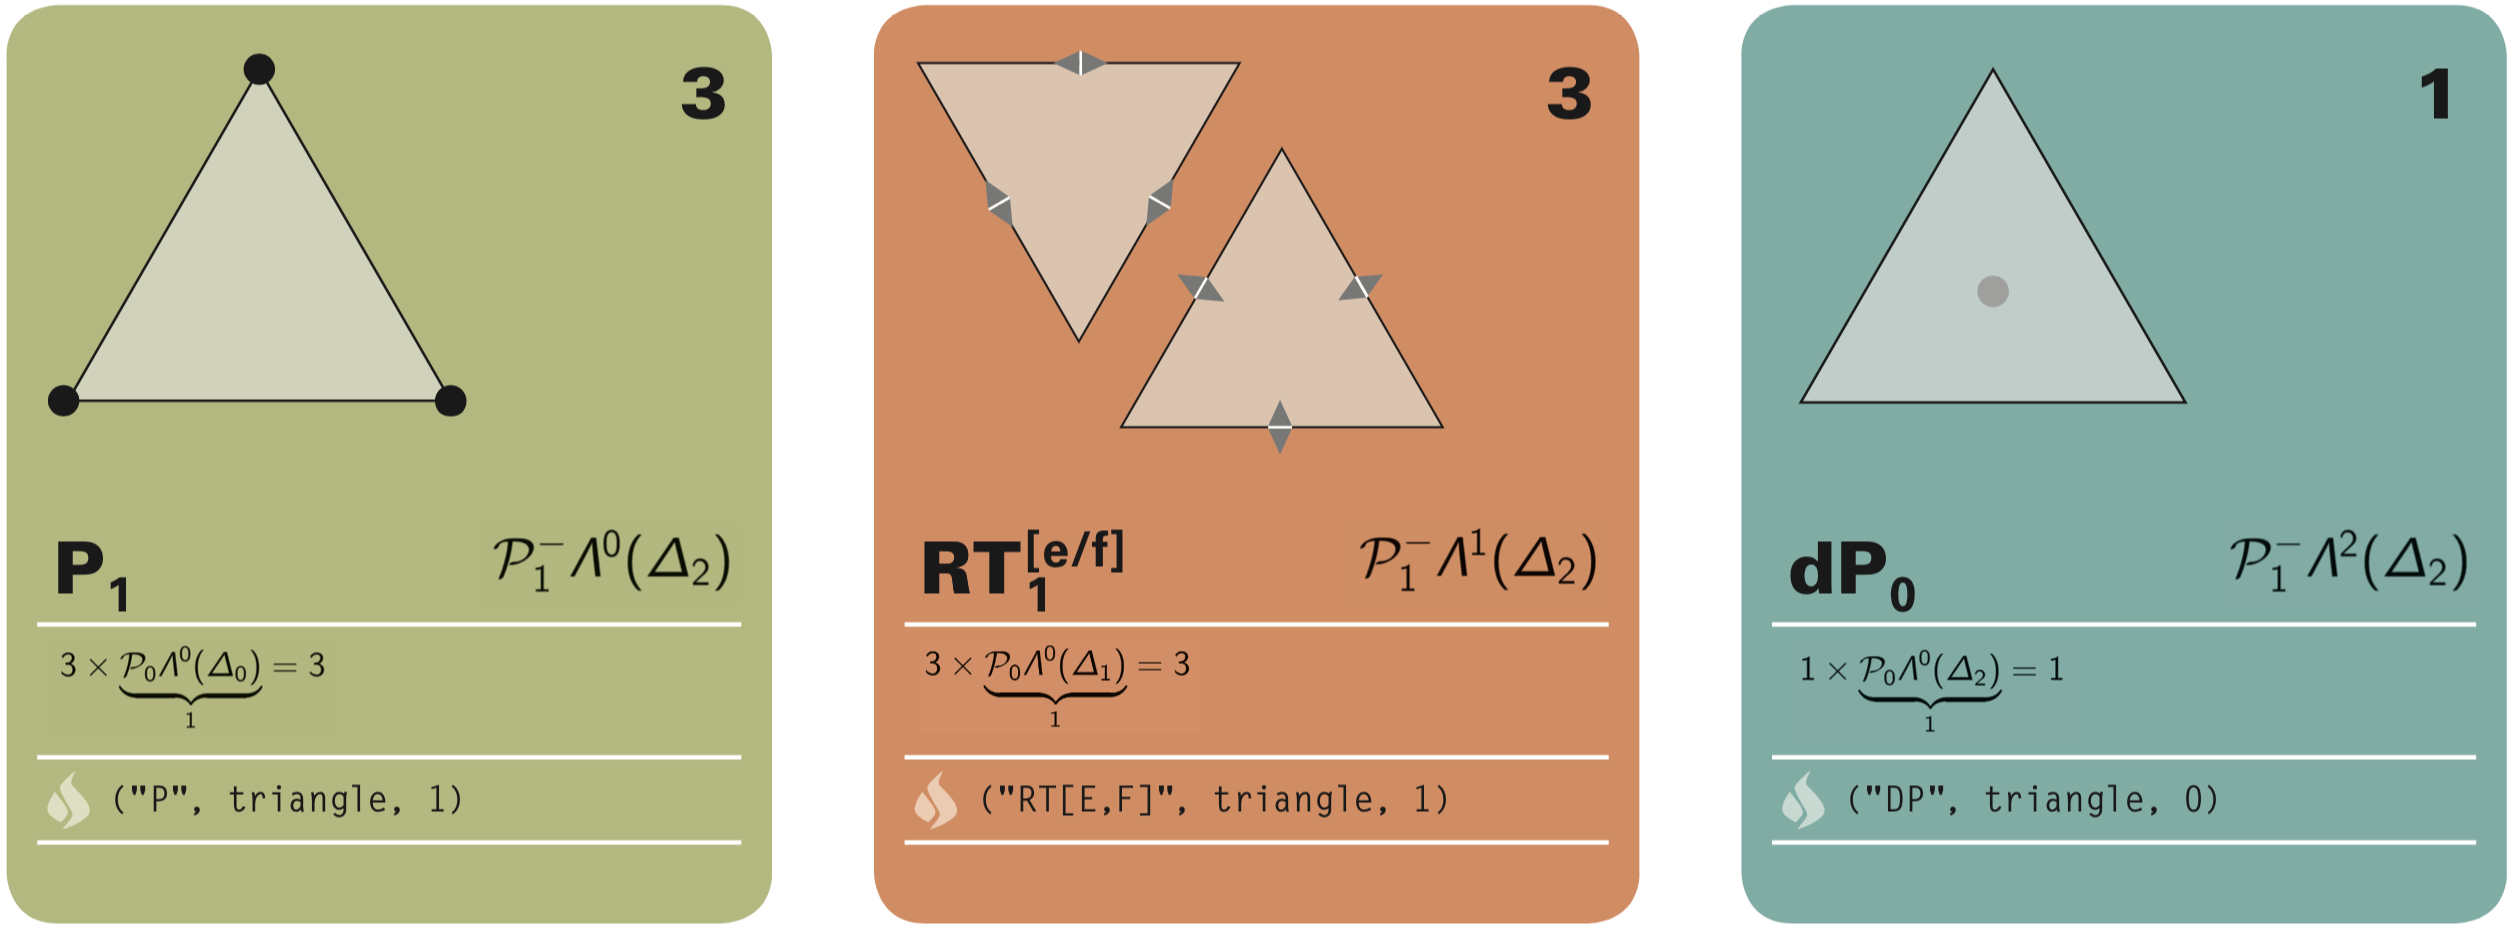
\includegraphics[width=0.5\textwidth]{rt-2d}
    \end{center}
    \vspace*{-\baselineskip}
    {\hfill \url{femtable.org}}
  \end{block}
  \pause
  \begin{columns}
    \begin{column}{0.7\textwidth}
      \begin{itemize}
      \item Exact sequence: $\ker(\div) = \range(\grad^\perp)$
      \item Need patches containing support of the $P_k$ basis
        functions $\Rightarrow$ star around vertices
      \end{itemize}
    \end{column}
    \begin{column}{0.3\textwidth}
      \begin{tikzpicture}[scale=2,
        on each segment/.style={
          decorate,
          decoration={
            show path construction,
            moveto code={},
            lineto code={
              \path [#1]
              (\tikzinputsegmentfirst) -- (\tikzinputsegmentlast);
            }}},
        dof/.style={postaction={decorate, decoration={markings,
              mark=at position 0.5 with {
                \node[transform shape,shape=diamond,fill,draw, inner
                sep=0pt, minimum height=5pt, minimum width=2.5pt] {};
              }}}}]
        \foreach \i/\k in {0/0, 0.5/1, 1/2} {
          \foreach \j/\l in {0/0, 0.5/1, 1/2} {
            \coordinate (v\k\l) at (\i, \j);
          }
        }

        \draw[thick, black, line join=miter, postaction={on each segment={dof}}] (v00)
        -- (v10) -- (v20) -- (v21) -- (v22) -- (v12) -- (v02) -- (v01) -- (v00);
        \draw[dof, thick, black, line join=cap] (v01) -- (v11);
        \draw[dof, thick, black, line join=cap] (v11) -- (v21);
        \draw[dof, thick, black, line join=cap] (v10) -- (v11);
        \draw[dof, thick, black, line join=cap] (v11) -- (v12);
        \draw[dof, thick, black, line join=cap] (v01) -- (v10);
        \draw[dof, thick, black, line join=cap] (v02) -- (v11);
        \draw[dof, thick, black, line join=cap] (v11) -- (v20);
        \draw[dof, thick, black, line join=cap] (v12) -- (v21);
        \coordinate (i10) at ($(v10) + (90:0.05)$);
        \coordinate (i20) at ($(v20) + (135:0.07071)$);
        \coordinate (i21) at ($(v21) + (180:0.05)$);
        \coordinate (i12) at ($(v12) + (270:0.05)$);
        \coordinate (i02) at ($(v02) + (315:0.07071)$);
        \coordinate (i01) at ($(v01) + (0:0.05)$);
        \begin{scope}[on background layer]
          \path[fill=cyan] \convexpath{i01,i02,i12,i21,i20,i10}{0.5pt};
        \end{scope}
      \end{tikzpicture}
    \end{column}
  \end{columns}
\end{frame}

\begin{frame}[fragile, t]
  \frametitle{{$H(\div)$ multigrid in 2D {\small \parencite{Arnold:1997}}}}
  \vspace*{-1.5\baselineskip}
  \begin{equation*}
    \text{Find $u \in V \subset H(\div)$ s.t.}\quad (u, v) + \gamma (\div u, \div v) = (f, v) \quad \forall v \in V.
  \end{equation*}
  \vspace{-\baselineskip}
  \begin{columns}
    \begin{column}{0.7\textwidth}
      {\scriptsize
\begin{verbatim}
    -ksp_type cg
    -pc_type mg
    -mg_levels_
       -pc_type python
       -pc_python_type firedrake.PatchPC
       -patch_
          -pc_patch_construct_dim 0
          -pc_patch_construct_type star
\end{verbatim}
}
    \end{column}
    \begin{column}{0.3\textwidth}
      \begin{center}
      \begin{tikzpicture}[scale=2,
        on each segment/.style={
          decorate,
          decoration={
            show path construction,
            moveto code={},
            lineto code={
              \path [#1]
              (\tikzinputsegmentfirst) -- (\tikzinputsegmentlast);
            }}},
        dof/.style={postaction={decorate, decoration={markings,
              mark=at position 0.5 with {
                \node[transform shape,shape=diamond,fill,draw, inner
                sep=0pt, minimum height=5pt, minimum width=2.5pt] {};
              }}}}]
        \foreach \i/\k in {0/0, 0.5/1, 1/2} {
          \foreach \j/\l in {0/0, 0.5/1, 1/2} {
            \coordinate (v\k\l) at (\i, \j);
          }
        }

        \draw[thick, black, line join=miter, postaction={on each segment={dof}}] (v00)
        -- (v10) -- (v20) -- (v21) -- (v22) -- (v12) -- (v02) -- (v01)
        -- (v00);
        \draw[dof, thick, black, line join=cap] (v01) -- (v11);
        \draw[dof, thick, black, line join=cap] (v11) -- (v21);
        \draw[dof, thick, black, line join=cap] (v10) -- (v11);
        \draw[dof, thick, black, line join=cap] (v11) -- (v12);
        \draw[dof, thick, black, line join=cap] (v01) -- (v10);
        \draw[dof, thick, black, line join=cap] (v02) -- (v11);
        \draw[dof, thick, black, line join=cap] (v11) -- (v20);
        \draw[dof, thick, black, line join=cap] (v12) -- (v21);
        \coordinate (i10) at ($(v10) + (90:0.05)$);
        \coordinate (i20) at ($(v20) + (135:0.07071)$);
        \coordinate (i21) at ($(v21) + (180:0.05)$);
        \coordinate (i12) at ($(v12) + (270:0.05)$);
        \coordinate (i02) at ($(v02) + (315:0.07071)$);
        \coordinate (i01) at ($(v01) + (0:0.05)$);
        \begin{scope}[on background layer]
          \path[fill=cyan]
          \convexpath{i01,i02,i12,i21,i20,i10}{0.5pt};
        \end{scope}
      \end{tikzpicture}
      \end{center}
    \end{column}
  \end{columns}    

  \begin{center}
    \begin{table}
      \begin{tabular}{l|cccccc}
        Smoother\hfill$\gamma$ & $0$ & $10^{-1}$ & $10^{0}$ & $10^{1}$ & $10^{2}$ & $10^{3}$ \\
        \midrule
        Point-Jacobi ($k=1$)  & 11 & 27 &  49 &68 &  86 & 103  \\
        Point-Jacobi  ($k=2$) & 10 & 45 &  71 & 93 & 113 & 134 \\
        \midrule
        Block-Jacobi  ($k=1$) &  6 & 11 &  12 & 12  &  12 & 12 \\
        Block-Jacobi  ($k=2$) &  7 & 8  &   8 & 8   &   8 & 8 
      \end{tabular}
      \caption{Iteration counts for multigrid preconditioned CG using
        $\text{RT}_k$ elements.}
    \end{table}
  \end{center}
\end{frame}

\begin{frame}[fragile,t]
  \frametitle{$H(\div)$ and $H(\curl)$ multigrid in 3D
    {\small \parencite{Arnold:2000}}}
  \vspace{-1.5\baselineskip}
  \begin{equation*}
    \text{Find $u \in V \subset H(\curl)$ s.t.}\quad (u, v) + \gamma (\curl u, \curl v) = (f, v) \quad \forall v \in V.
  \end{equation*}
  \vspace*{-\baselineskip}
  \begin{block}{$L^2$ de Rham complex}
    \begin{equation*}
      H^1 \xrightarrow{\grad} H(\curl) \xrightarrow{\curl} H(\div) \xrightarrow{\div} L^2
    \end{equation*}
    \vspace*{-2\baselineskip}
    \pause
    \begin{center}
      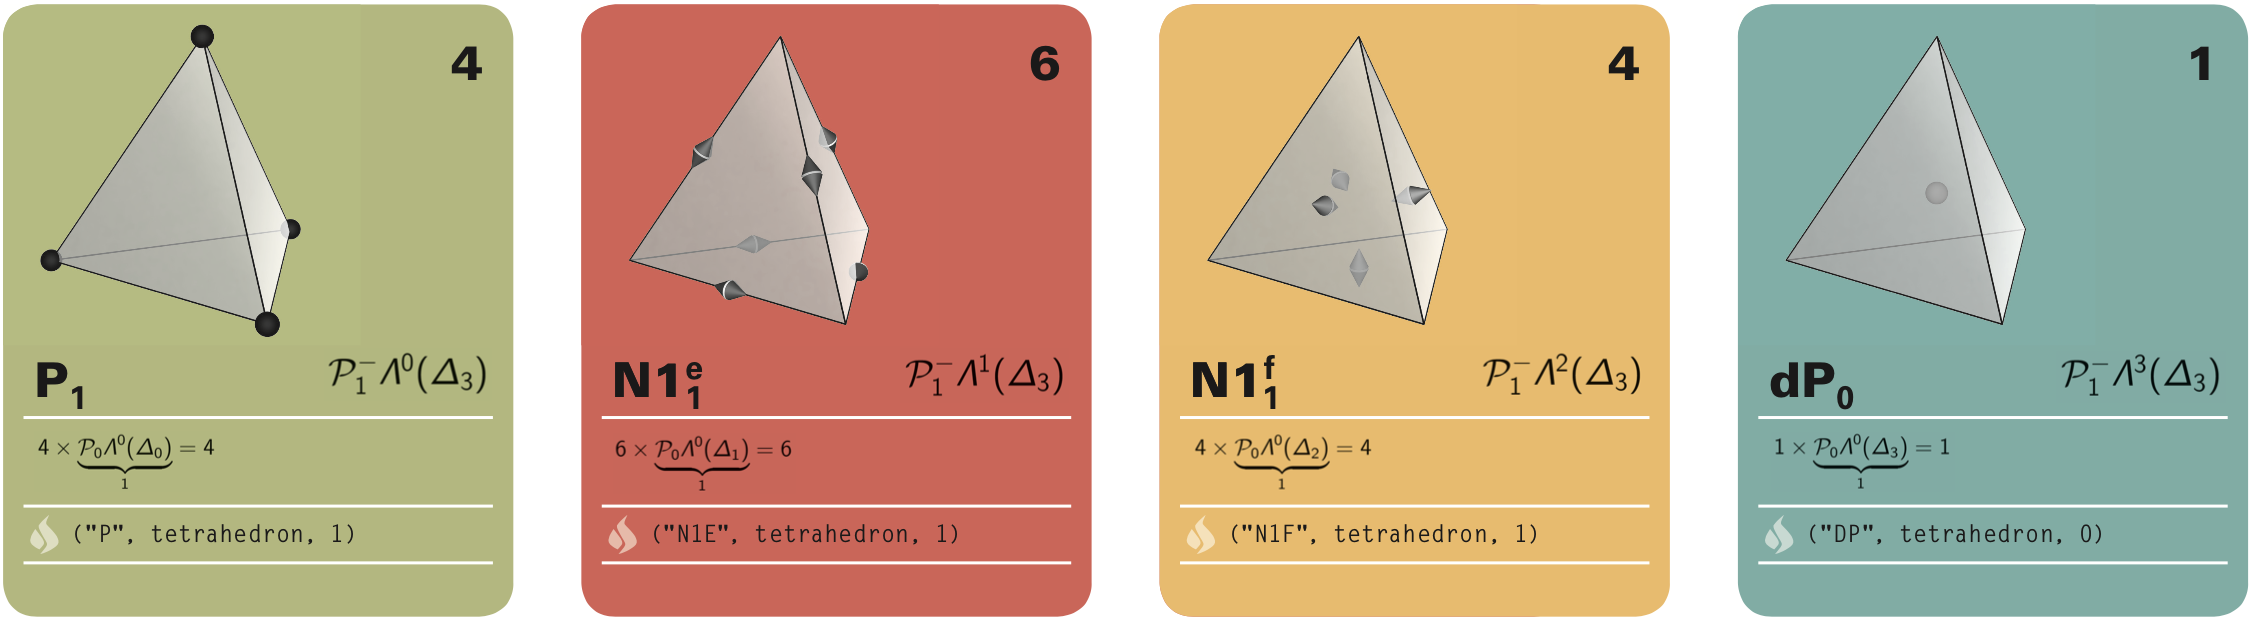
\includegraphics[width=0.5\textwidth]{rt-3d}
    \end{center}
    \vspace*{-\baselineskip}
    {\hfill \url{femtable.org}}
  \end{block}
  \begin{columns}
    \begin{column}{0.5\textwidth}
      \begin{itemize}
      \item Exact sequence: $\ker(\curl) = \range(\grad)$, $\ker(\div)
        = \range(\curl)$
      \item $H(\curl)$: star around vertices
      \item $H(\div)$: star around edges
      \end{itemize}
    \end{column}
    \begin{column}{0.5\textwidth}
      \begin{center}
      \begin{tikzpicture}[scale=2,
        on each segment/.style={
          decorate,
          decoration={
            show path construction,
            moveto code={},
            lineto code={
              \path [#1]
              (\tikzinputsegmentfirst) -- (\tikzinputsegmentlast);
            }}},
        nedof/.style={postaction={decorate, decoration={markings,
              mark=at position 0.5 with {
                \node[transform shape,shape=diamond,fill,draw, inner
                sep=0pt, minimum height=2.5pt, minimum width=5pt] {};
              }}}},
        rtdof/.style={postaction={decorate, decoration={markings,
              mark=at position 0.5 with {
                \node[transform shape,shape=diamond,fill,draw, inner
                sep=0pt, minimum height=5pt, minimum width=2.55pt] {};
              }}}}]
        \foreach \i/\k in {0/0, 0.5/1, 1/2} {
          \foreach \j/\l in {0/0, 0.5/1, 1/2} {
            \coordinate (v\k\l) at (\i, \j);
          }
        }

        \draw[thick, black, line join=miter, postaction={on each segment={nedof}}] (v00)
        -- (v10) -- (v20) -- (v21) -- (v22) -- (v12) -- (v02) -- (v01)
        -- (v00);
        \draw[nedof, thick, black, line join=cap] (v01) -- (v11);
        \draw[nedof, thick, black, line join=cap] (v11) -- (v21);
        \draw[nedof, thick, black, line join=cap] (v10) -- (v11);
        \draw[nedof, thick, black, line join=cap] (v11) -- (v12);
        \draw[nedof, thick, black, line join=cap] (v01) -- (v10);
        \draw[nedof, thick, black, line join=cap] (v02) -- (v11);
        \draw[nedof, thick, black, line join=cap] (v11) -- (v20);
        \draw[nedof, thick, black, line join=cap] (v12) -- (v21);
        \coordinate (i10) at ($(v10) + (90:0.05)$);
        \coordinate (i20) at ($(v20) + (135:0.07071)$);
        \coordinate (i21) at ($(v21) + (180:0.05)$);
        \coordinate (i12) at ($(v12) + (270:0.05)$);
        \coordinate (i02) at ($(v02) + (315:0.07071)$);
        \coordinate (i01) at ($(v01) + (0:0.05)$);
        \begin{scope}[on background layer]
          \path[fill=cyan]
          \convexpath{i01,i02,i12,i21,i20,i10}{0.5pt};
        \end{scope}
        \begin{scope}[shift={(1.5, 0)}]
          \foreach \i/\k in {0/0, 0.5/1, 1/2} {
            \foreach \j/\l in {0/0, 0.5/1, 1/2} {
              \coordinate (v\k\l) at (\i, \j);
            }
          }
          \draw[thick, black, line join=miter, postaction={on each segment={rtdof}}] (v00)
          -- (v10) -- (v20) -- (v21) -- (v22) -- (v12) -- (v02) -- (v01)
          -- (v00);
          \draw[rtdof, thick, black, line join=cap] (v01) -- (v11);
          \draw[rtdof, thick, black, line join=cap] (v11) -- (v21);
          \draw[rtdof, thick, black, line join=cap] (v10) -- (v11);
          \draw[rtdof, thick, black, line join=cap] (v11) -- (v12);
          \draw[rtdof, thick, black, line join=cap] (v01) -- (v10);
          \draw[rtdof, thick, black, line join=cap] (v02) -- (v11);
          \draw[rtdof, thick, black, line join=cap] (v11) -- (v20);
          \draw[rtdof, thick, black, line join=cap] (v12) -- (v21);


          \coordinate (e00) at ($(v00) + (45:0.07071)$);
          \coordinate (e10) at ($(v10) + (135:0.07071)$);
          \coordinate (e11) at ($(v11) + (225:0.07071)$);
          \coordinate (e01) at ($(v01) + (315:0.07071)$);

          \begin{scope}[on background layer]
            \path[fill=cyan]
            \convexpath{e00,e01,e11,e10}{0pt};
          \end{scope}
          \coordinate (o11) at ($(v11) + (90:0.03535)$);
          \coordinate (o21) at ($(v21) + (157.5:0.1)$);
          \coordinate (o12) at ($(v12) + (270:0.03535)$);
          \coordinate (o02) at ($(v02) + (337.5:0.1)$);

          \begin{scope}[on background layer]
            \path[fill=cyan]
            \convexpath{o11,o02,o12,o21}{0pt};
          \end{scope}
        \end{scope}
      \end{tikzpicture}
      \end{center}
    \end{column}
  \end{columns}
\end{frame}

\begin{frame}[fragile,t]
  \frametitle{$H(\curl)$ multigrid in 3D {\small \parencite{Arnold:2000}}}
  \vspace{-1.5\baselineskip}
  \begin{equation*}
    \text{Find $u \in V \subset H(\curl)$ s.t.}\quad (u, v) + \gamma (\curl u, \curl v) = (f, v) \quad \forall v \in V.
  \end{equation*}
  \vspace*{-\baselineskip}
  \begin{columns}
    \begin{column}{0.7\textwidth}
      {\scriptsize
\begin{verbatim}
    -ksp_type cg
    -pc_type mg
    -mg_levels_
       -pc_type python
       -pc_python_type firedrake.PatchPC
       -patch_
          -pc_patch_construct_dim 0
          -pc_patch_construct_type star
\end{verbatim}
      }
    \end{column}
    \begin{column}{0.3\textwidth}
      \begin{center}
        \begin{tikzpicture}[scale=2,
          on each segment/.style={
            decorate,
            decoration={
              show path construction,
              moveto code={},
              lineto code={
                \path [#1]
                (\tikzinputsegmentfirst) -- (\tikzinputsegmentlast);
              }}},
          dof/.style={postaction={decorate, decoration={markings,
                mark=at position 0.5 with {
                  \node[transform shape,shape=diamond,fill,draw, inner
                  sep=0pt, minimum height=2.5pt, minimum width=5pt] {};
                }}}}]
          \foreach \i/\k in {0/0, 0.5/1, 1/2} {
            \foreach \j/\l in {0/0, 0.5/1, 1/2} {
              \coordinate (v\k\l) at (\i, \j);
            }
          }

          \draw[thick, black, line join=miter, postaction={on each segment={dof}}] (v00)
          -- (v10) -- (v20) -- (v21) -- (v22) -- (v12) -- (v02) -- (v01)
          -- (v00);
          \draw[dof, thick, black, line join=cap] (v01) -- (v11);
          \draw[dof, thick, black, line join=cap] (v11) -- (v21);
          \draw[dof, thick, black, line join=cap] (v10) -- (v11);
          \draw[dof, thick, black, line join=cap] (v11) -- (v12);
          \draw[dof, thick, black, line join=cap] (v01) -- (v10);
          \draw[dof, thick, black, line join=cap] (v02) -- (v11);
          \draw[dof, thick, black, line join=cap] (v11) -- (v20);
          \draw[dof, thick, black, line join=cap] (v12) -- (v21);
          \coordinate (i10) at ($(v10) + (90:0.05)$);
          \coordinate (i20) at ($(v20) + (135:0.07071)$);
          \coordinate (i21) at ($(v21) + (180:0.05)$);
          \coordinate (i12) at ($(v12) + (270:0.05)$);
          \coordinate (i02) at ($(v02) + (315:0.07071)$);
          \coordinate (i01) at ($(v01) + (0:0.05)$);
          \begin{scope}[on background layer]
            \path[fill=cyan]
            \convexpath{i01,i02,i12,i21,i20,i10}{0.5pt};
          \end{scope}
        \end{tikzpicture}
      \end{center}
    \end{column}
  \end{columns}    

  \begin{center}
    \begin{table}
      \begin{tabular}{l|cccccc}
        % Hcurl
        Smoother\hfill$\gamma$ & $0$ & $10^{-1}$ & $10^{0}$ & $10^{1}$ & $10^{2}$ & $10^{3}$ \\
        \midrule
        Point-Jacobi ($k=1$)  & 10 & 48  &  85 & 120 & 150 & 180 \\
        Point-Jacobi  ($k=2$) & 22 & 115 & 211 & 293 & 370 & 446 \\
        \midrule
        Block-Jacobi  ($k=1$) &  9 & 16  &  18 & 18  &  18 & 18  \\
        Block-Jacobi  ($k=2$) &  9 & 12  &  12 & 12  &  12 & 12 
      \end{tabular}
      \caption{Iteration counts for multigrid preconditioned CG using Nedelec edge-elements of the first kind.}
    \end{table}
  \end{center}
\end{frame}

\begin{frame}[fragile,t]
  \frametitle{$H(\div)$ multigrid in 3D {\small \parencite{Arnold:2000}}}
  \vspace{-1.5\baselineskip}
  \begin{equation*}
    \text{Find $u \in V \subset H(\div)$ s.t.}\quad (u, v) + \gamma (\div u, \div v) = (f, v) \quad \forall v \in V.
  \end{equation*}
  \vspace*{-\baselineskip}
  \begin{columns}
    \begin{column}{0.7\textwidth}
      {\scriptsize
\begin{verbatim}
    -ksp_type cg
    -pc_type mg
    -mg_levels_
       -pc_type python
       -pc_python_type firedrake.PatchPC
       -patch_
          -pc_patch_construct_dim 1
          -pc_patch_construct_type star
\end{verbatim}
      }
    \end{column}
    \begin{column}{0.3\textwidth}
      \begin{center}
        \begin{tikzpicture}[scale=2,
          on each segment/.style={
            decorate,
            decoration={
              show path construction,
              moveto code={},
              lineto code={
                \path [#1]
                (\tikzinputsegmentfirst) -- (\tikzinputsegmentlast);
              }}},
          dof/.style={postaction={decorate, decoration={markings,
                mark=at position 0.5 with {
                  \node[transform shape,shape=diamond,fill,draw, inner
                  sep=0pt, minimum height=5pt, minimum width=2.5pt] {};
                }}}}]
          \foreach \i/\k in {0/0, 0.5/1, 1/2} {
            \foreach \j/\l in {0/0, 0.5/1, 1/2} {
              \coordinate (v\k\l) at (\i, \j);
            }
          }

          \draw[thick, black, line join=miter, postaction={on each segment={dof}}] (v00)
          -- (v10) -- (v20) -- (v21) -- (v22) -- (v12) -- (v02) -- (v01)
          -- (v00);
          \draw[dof, thick, black, line join=cap] (v01) -- (v11);
          \draw[dof, thick, black, line join=cap] (v11) -- (v21);
          \draw[dof, thick, black, line join=cap] (v10) -- (v11);
          \draw[dof, thick, black, line join=cap] (v11) -- (v12);
          \draw[dof, thick, black, line join=cap] (v01) -- (v10);
          \draw[dof, thick, black, line join=cap] (v02) -- (v11);
          \draw[dof, thick, black, line join=cap] (v11) -- (v20);
          \draw[dof, thick, black, line join=cap] (v12) -- (v21);


          \coordinate (e00) at ($(v00) + (45:0.07071)$);
          \coordinate (e10) at ($(v10) + (135:0.07071)$);
          \coordinate (e11) at ($(v11) + (225:0.07071)$);
          \coordinate (e01) at ($(v01) + (315:0.07071)$);

          \begin{scope}[on background layer]
            \path[fill=cyan]
            \convexpath{e00,e01,e11,e10}{0pt};
          \end{scope}

          \coordinate (o11) at ($(v11) + (90:0.03535)$);
          \coordinate (o21) at ($(v21) + (157.5:0.1)$);
          \coordinate (o12) at ($(v12) + (270:0.03535)$);
          \coordinate (o02) at ($(v02) + (337.5:0.1)$);

          \begin{scope}[on background layer]
            \path[fill=cyan]
            \convexpath{o11,o02,o12,o21}{0pt};
          \end{scope}
        \end{tikzpicture}
      \end{center}
    \end{column}
  \end{columns}    
  \begin{center}
    \begin{table}
      \begin{tabular}{l|cccccc}
        % Hdiv
        Smoother\hfill$\gamma$ & $0$ & $10^{-1}$ & $10^{0}$ & $10^{1}$ & $10^{2}$ & $10^{3}$ \\
        \midrule
        Point-Jacobi ($k=1$)  & 11 & 63  & 109 & 146 & 180 & 221 \\
        Point-Jacobi  ($k=2$) & 26 & 180 & 366 & 531 & 687 & 844 \\
        \midrule
        Block-Jacobi  ($k=1$) & 12 & 30  &  36 & 36  &  37 & 37  \\
        Block-Jacobi  ($k=2$) & 11 & 17  &  17 & 17  &  17 & 17
      \end{tabular}
      \caption{Iteration counts for multigrid preconditioned CG using Nedelec face-elements of the first kind.}
    \end{table}
    \end{center}
\end{frame}

\begin{frame}[fragile,t]
  \frametitle{Nearly incompressible elasticity {\footnotesize \parencite{Farrell:2020}}}
  \vspace*{-1.5\baselineskip}
  \begin{equation*}
    \text{Find $u \in V \subset H^1$ s.t.} \quad (\grad u, \grad v) + \gamma (\div u, \div v) = (f, v) \quad \forall v \in V.
  \end{equation*}
  \vspace*{-\baselineskip}
  \begin{block}{2D Stokes complex}
    \begin{equation*}
      H^2 \xrightarrow{\grad^\perp} H^1 \xrightarrow{\div} L^2
    \end{equation*}
    \vspace*{-\baselineskip}
    \begin{center}
      \includestandalone[width=0.5\textwidth]{./../pictures/HCT-complex}
    \end{center}
    \begin{itemize}
    \item Decomposition must capture $\ker \div = \range \grad^\perp$.
    \item Support of HCT element is on ``macro'' mesh $\Rightarrow$ \texttt{macrostar}
    \end{itemize}
  \end{block}
\end{frame}
\begin{frame}[t, fragile]
  \frametitle{Nearly incompressible elasticity {\footnotesize \parencite{Farrell:2020}}}
  \begin{onlyenv}<1-3>
    \begin{center}
      \begin{tikzpicture}[scale=2,
        bcdof/.style={postaction={decorate,decoration={markings,
              mark=at position 0.5 with {\draw[solid, fill, black!60] circle
                (0.06);}}}},
        dof/.style={postaction={decorate,decoration={markings,
              mark=at position 0.5 with {\draw[solid, fill, black] circle (0.06);}}}
        }]

        \foreach \i in {0, 1, 2, 3} {
          \coordinate (0-\i) at ($(\i*1.5, 0)$);
          \coordinate (1-\i) at ($(0-\i) + (60:1.5)$);
          \coordinate (2-\i) at ($(1-\i) + (120:1.5)$);
        }
        \foreach \i/\j in {0/1, 1/2, 2/3} {
          \foreach \k in {0, 2} {
            \draw[line join=miter, very thick] (\k-\i) -- (\k-\j);
          }
          \draw[line join=miter, very thick] (0-\i) -- (1-\i);
          \draw[line join=miter, very thick] (1-\i) -- (2-\i);
          \draw[line join=miter, very thick] (0-\j) -- (1-\i);
          \draw[line join=miter, very thick] (1-\i) -- (2-\j);
        }

        \foreach \i/\j in {0/1, 1/2} {
          \draw[line join=miter, very thick] (1-\i) -- (1-\j);
        }
        \begin{scope}[on background layer]
          \path[fill=cyan] 
          ([shift={(0:4pt)}]1-0) --
          ([shift={(60:4pt)}]0-1) --
          ([shift={(120:4pt)}]0-2) --
          ([shift={(180:4pt)}]1-2) --
          ([shift={(240:4pt)}]2-2) --
          ([shift={(300:4pt)}]2-1) -- cycle;
        \end{scope}
        \pause

        \foreach \i/\j in {0/1, 1/2, 2/3} {
          \coordinate (bc-0-\i-\j) at (barycentric cs:0-\i=1,0-\j=1,1-\i=1);
          \draw[line join=miter, very thick] (0-\i) -- (bc-0-\i-\j);
          \draw[line join=miter, very thick] (1-\i) -- (bc-0-\i-\j);
          \draw[line join=miter, very thick] (0-\j) -- (bc-0-\i-\j);

          \coordinate (bc-2-\i-\j) at (barycentric cs:1-\i=1,2-\i=1,2-\j=1);
          \draw[line join=miter, very thick] (1-\i) -- (bc-2-\i-\j);
          \draw[line join=miter, very thick] (2-\i) -- (bc-2-\i-\j);
          \draw[line join=miter, very thick] (2-\j) -- (bc-2-\i-\j);
        }
        \foreach \i/\j in {0/1, 1/2} { 
          \coordinate (bc-1-\i-\j)  at (barycentric cs:1-\i=1,0-\j=1,1-\j=1);
          \draw[line join=miter, very thick] (1-\i) -- (bc-1-\i-\j);
          \draw[line join=miter, very thick] (0-\j) -- (bc-1-\i-\j);
          \draw[line join=miter, very thick] (1-\j) -- (bc-1-\i-\j);

          \coordinate (bc-3-\i-\j)  at (barycentric cs:1-\i=1,1-\j=1,2-\j=1);
          \draw[line join=miter, very thick] (1-\i) -- (bc-3-\i-\j);
          \draw[line join=miter, very thick] (1-\j) -- (bc-3-\i-\j);
          \draw[line join=miter, very thick] (2-\j) -- (bc-3-\i-\j);
        }

        \pause

        \foreach \i in {0, 1, 2, 3} {
          \foreach \j in {0, 2} {
            \draw[fill, black] (\j-\i) circle (0.05);
          }
        }
        \foreach \i in {0, 1, 2} {
          \draw[fill] (1-\i) circle (0.05);
        }
        \foreach \i/\j in {0/1, 1/2, 2/3} {
          \foreach \k in {0, 2} {
            \draw[fill] (bc-\k-\i-\j) circle (0.05);
          }
        }
        \foreach \i/\j in {0/1, 1/2} { 
          \foreach \k in {1, 3} {
            \draw[fill] (bc-\k-\i-\j) circle (0.05);
          }
        }

        \foreach \i/\j in {0/1, 1/2, 2/3} {
          \draw[fill] (barycentric cs:0-\i=1,0-\j=1) circle (0.05);
          \draw[fill] (barycentric cs:2-\i=1,2-\j=1) circle (0.05);
          \draw[fill] (barycentric cs:0-\i=1,1-\i=1) circle (0.05);
          \draw[fill] (barycentric cs:0-\j=1,1-\i=1) circle (0.05);
          \draw[fill] (barycentric cs:1-\i=1,2-\i=1) circle (0.05);
          \draw[fill] (barycentric cs:1-\i=1,2-\j=1) circle (0.05);
        }
        \draw[fill] (barycentric cs:1-0=1,1-1=1) circle (0.05);
        \draw[fill] (barycentric cs:1-1=1,1-2=1) circle (0.05);

        \foreach \i in {0-0, 0-1, 1-0} {
          \draw[fill] (barycentric cs:\i=1,bc-0-0-1=1) circle (0.05);
        }
        \foreach \i in {0-1, 0-2, 1-1} {
          \draw[fill] (barycentric cs:\i=1,bc-0-1-2=1) circle (0.05);
        }
        \foreach \i in {0-2, 0-3, 1-2} {
          \draw[fill] (barycentric cs:\i=1,bc-0-2-3=1) circle (0.05);
        }
        \foreach \i in {2-0, 2-1, 1-0} {
          \draw[fill] (barycentric cs:\i=1,bc-2-0-1=1) circle (0.05);
        }
        \foreach \i in {2-1, 2-2, 1-1} {
          \draw[fill] (barycentric cs:\i=1,bc-2-1-2=1) circle (0.05);
        }
        \foreach \i in {2-2, 2-3, 1-2} {
          \draw[fill] (barycentric cs:\i=1,bc-2-2-3=1) circle (0.05);
        }
        \foreach \i in {0-1, 1-0, 1-1} {
          \draw[fill] (barycentric cs:\i=1,bc-1-0-1=1) circle (0.05);
        }
        \foreach \i in {0-2, 1-1, 1-2} {
          \draw[fill] (barycentric cs:\i=1,bc-1-1-2=1) circle (0.05);
        }
        \foreach \i in {1-0, 2-1, 1-1} {
          \draw[fill] (barycentric cs:\i=1,bc-3-0-1=1) circle (0.05);
        }
        \foreach \i in {1-1, 2-2, 1-2} {
          \draw[fill] (barycentric cs:\i=1,bc-3-1-2=1) circle (0.05);
        }
      \end{tikzpicture}
    \end{center}
  \end{onlyenv}
  \begin{onlyenv}<4->
    \vspace*{-1.5\baselineskip}
    \begin{equation*}
      \text{Find $u \in V \subset H^1$ s.t.} \quad (\grad u, \grad v) + \gamma (\div u, \div v) = (f, v) \quad \forall v \in V.
    \end{equation*}
    \vspace*{-1.5\baselineskip}
    \begin{columns}
      \begin{column}{0.7\textwidth}
\begin{minted}[fontsize=\scriptsize]{text}
-ksp_type cg
-pc_type mg
-mg_levels_
  -pc_type python
  -pc_python_type firedrake.PatchPC
    -patch_
      -pc_patch_construct_dim 0
      -pc_patch_construct_type python
      -pc_patch_construct_python_type macrostar
\end{minted}
      \end{column}
      \begin{column}{0.3\textwidth}
        \begin{tikzpicture}[scale=1,
          dof/.style={blue, postaction={decorate,decoration={markings,
          mark=at position 0.5 with {\draw[solid, fill=blue, blue] circle (0.06);}}}
          }]
          \coordinate (0-0) at (1.5, 0);
          \coordinate (0-1) at (3, 0);
          \coordinate (1-0) at ($(0-0) + (120:1.5)$);
          \coordinate (1-1) at ($(1-0) + (1.5, 0)$);
          \coordinate (1-2) at ($(1-0) + (3, 0)$);
          \coordinate (2-0) at ($(1-0) + (60:1.5)$);
          \coordinate (2-1) at ($(2-0) + (1.5, 0)$);
          \foreach \i in {0, 1, 2} {
          \foreach \j in {0, 1} {
          \draw[fill=blue, blue] (\i-\j) circle (0.06);
          }
          }
          \draw[fill=blue, blue] (1-2) circle (0.06);

          \coordinate (bc0) at (barycentric cs:0-0=1,1-0=1,1-1=1);
          \coordinate (bc1) at (barycentric cs:0-0=1,0-1=1,1-1=1);
          \coordinate (bc2) at (barycentric cs:0-1=1,1-1=1,1-2=1);
          \coordinate (bc3) at (barycentric cs:1-0=1,1-1=1,2-0=1);
          \coordinate (bc4) at (barycentric cs:1-1=1,2-0=1,2-1=1);
          \coordinate (bc5) at (barycentric cs:1-1=1,2-1=1,1-2=1);
          \foreach \i in {0, 1, 2, 3, 4, 5} {
          \draw[fill=blue, blue] (bc\i) circle (0.06);
          }

          \draw[dof, line join=miter, thick] (0-0) -- (0-1);
          \draw[dof, line join=miter, thick] (0-1) -- (1-2);
          \draw[dof, line join=miter, thick] (1-2) -- (2-1);
          \draw[dof, line join=miter, thick] (2-1) -- (2-0);
          \draw[dof, line join=miter, thick] (2-0) -- (1-0);
          \draw[dof, line join=miter, thick] (1-0) -- (0-0);

          \draw[dof, line join=miter, thick] (0-0) -- (1-1);
          \draw[dof, line join=miter, thick] (0-1) -- (1-1);
          \draw[dof, line join=miter, thick] (1-0) -- (1-1);
          \draw[dof, line join=miter, thick] (1-2) -- (1-1);
          \draw[dof, line join=miter, thick] (2-0) -- (1-1);
          \draw[dof, line join=miter, thick] (2-1) -- (1-1);

          \draw[dof, line join=miter, thick] (0-0) -- (bc0);
          \draw[dof, line join=miter, thick] (1-0) -- (bc0);
          \draw[dof, line join=miter, thick] (1-1) -- (bc0);

          \draw[dof, line join=miter, thick] (0-0) -- (bc1);
          \draw[dof, line join=miter, thick] (0-1) -- (bc1);
          \draw[dof, line join=miter, thick] (1-1) -- (bc1);

          \draw[dof, line join=miter, thick] (0-1) -- (bc2);
          \draw[dof, line join=miter, thick] (1-2) -- (bc2);
          \draw[dof, line join=miter, thick] (1-1) -- (bc2);

          \draw[dof, line join=miter, thick] (2-0) -- (bc3);
          \draw[dof, line join=miter, thick] (1-0) -- (bc3);
          \draw[dof, line join=miter, thick] (1-1) -- (bc3);

          \draw[dof, line join=miter, thick] (2-1) -- (bc4);
          \draw[dof, line join=miter, thick] (2-0) -- (bc4);
          \draw[dof, line join=miter, thick] (1-1) -- (bc4);

          \draw[dof, line join=miter, thick] (1-2) -- (bc5);
          \draw[dof, line join=miter, thick] (2-1) -- (bc5);
          \draw[dof, line join=miter, thick] (1-1) -- (bc5);
          \begin{scope}[on background layer]
            \draw[cyan, fill=cyan] ([shift={(60:5pt)}]0-0) --
            ([shift={(120:5pt)}]0-1) --
            ([shift={(180:5pt)}]1-2) --
            ([shift={(240:5pt)}]2-1) --
            ([shift={(300:5pt)}]2-0) --
            ([shift={(0:5pt)}]1-0) --
            cycle;
          \end{scope}
        \end{tikzpicture}
      \end{column}
    \end{columns}
    \begin{overlayarea}{\textwidth}{0.275\textheight}
      \begin{onlyenv}<4>
        \vspace{0.5\baselineskip}
\begin{minted}[fontsize=\scriptsize]{python}
def macrostar(mesh, vertex):
    if not macro_vertex(vertex):
        return None
    s = mesh.star(vertex)
    c = concat(*map(mesh.closure, s))
    macro_vertices = remove_if_not(macro_vertex, concat(s, *map(mesh.star(c))))
    return concat(s, *map(mesh.star, macro_vertices))
\end{minted}
      \end{onlyenv}
      \begin{onlyenv}<5->
        \begin{table}
          \centering
          \begin{tabular}{cr|cccccccc}
            \toprule
            levels & DoFs\hfill$\gamma$ & $10^0$ & $10^1$ & $10^2$ & $10^3$ & $10^4$ & $10^6$ & $10^8$ \\
            \midrule
            1      & $2.39 \times 10^4$ & 15     & 14     & 18     & 23     & 25     & 26     & 25     \\
            2      & $1.85\times 10^5$  & 16     & 16     & 21     & 26     & 29     & 31     & 30     \\
            3      & $1.46\times 10^6$  & 16     & 16     & 22     & 27     & 31     & 32     & 31     \\
            \bottomrule
          \end{tabular}
          \caption{Iteration counts in 3D for multigrid preconditioned
            CG with $\mathbb{P}_3^3$ elements}
          \label{tab:sv-elasticity}
        \end{table}
      \end{onlyenv}
    \end{overlayarea}
  \end{onlyenv}
\end{frame}

\begin{frame}[fragile, t]
  \frametitle{Monolithic (coupled) smoothers}
  Find $(u, p) \in V\times Q \subset (H^1)^d \times L^2$ s.t.
  \begin{equation*}
    \nu (\sym \grad u, \sym \grad v) - (p, \div v) - (\div u, q) = (f, v) \quad \forall (v, q) \in V \times Q.
  \end{equation*}

  \begin{answer}{Vanka patch \parencite{Vanka:1986,Farrell:2019c}}
    Solve simultaneously for $(u, p)$ on each pressure dof, gathering
    those velocity dofs that couple to the pressure dof.
    \vspace*{-0.5\baselineskip}
    \begin{itemize}
    \only<1-2>{\item \textbf{$(Q_k)^d-Q_{k-1}^{\text{disc}}$: loop over cells, gather closure of
          star}}
    \only<3->{\item $(Q_k)^d-Q_{k-1}^{\text{disc}}$: loop over cells, gather closure of star}
    \only<1-2>{\item $(P_k)^d-P_{k-1}$: loop over vertices, gather closure
      of star}
    \only<3->{\item \textbf{$(P_k)^d-P_{k-1}$: loop over vertices, gather closure of star}}
    \end{itemize}
  \end{answer}
  \vspace*{-1\baselineskip}
  \begin{overlayarea}{\textwidth}{0.52\textheight}
    \begin{onlyenv}<2>
      \begin{columns}[T]
        \begin{column}{0.5\textwidth}
          \begin{center}
            \begin{tikzpicture}[scale=0.87]
              \coordinate (0-0) at (0, 0);
              \coordinate (0-1) at ($({sin(60) * 1.5}, 0)$);
              \coordinate (0-2) at ($({sin(60) * 3}, 0)$);
              \coordinate (0-3) at ($({sin(60) * 4.5}, 0)$);
              \coordinate (1-0) at ($({sin(60) * 0}, {sin(60) * 1.5})$);
              \coordinate (1-1) at ($({sin(60) * 1.5}, {sin(60) * 1.5})$);
              \coordinate (1-2) at ($({sin(60) * 3}, {sin(60) * 1.5})$);
              \coordinate (1-3) at ($({sin(60) * 4.5}, {sin(60) * 1.5})$);
              \coordinate (2-0) at ($({sin(60) * 0}, {sin(60) * 3})$);
              \coordinate (2-1) at ($({sin(60) * 1.5}, {sin(60) * 3})$);
              \coordinate (2-2) at ($({sin(60) * 3}, {sin(60) * 3})$);
              \coordinate (2-3) at ($({sin(60) * 4.5}, {sin(60) * 3})$);

              \draw[blue, line join=miter, thick] (0-0) -- (0-1) --
              (0-2) -- (0-3) -- (1-3) -- (2-3) -- (2-2) -- (2-1) -- (2-0) -- (1-0) -- cycle;
              \draw[blue, line join=miter, thick] (1-0) -- (1-1) -- (1-2) -- (1-3);
              \draw[blue, line join=miter, thick] (0-1) -- (1-1) -- (2-1);
              \draw[blue, line join=miter, thick] (0-2) -- (1-2) -- (2-2);

              \foreach \i/\j in {0/1, 1/2, 2/3} {
              \foreach \k/\l in {0/1, 1/2} {
              \node[shape=rectangle, inner sep=0pt, minimum
              height=0.2cm, minimum width=0.2cm, red, fill=red] at
              (barycentric cs:\k-\i=1,\l-\i=1,\k-\j=1,\l-\j=1) {};
              }
              }

              \foreach \i in {0, 1, 2, 3} {
              \foreach \j in {0, 1, 2} {
              \draw[fill=blue, blue] (\j-\i) circle (0.1cm);
              }
              }
              \begin{scope}[on background layer]
                \draw[cyan, fill=cyan]
                ([shift={(45:-7pt)}]0-1) --
                ([shift={(135:-7pt)}]0-2) --
                ([shift={(225:-7pt)}]1-2) --
                ([shift={(315:-7pt)}]1-1) --
                cycle;
              \end{scope}
            \end{tikzpicture}
          \end{center}
        \end{column}
        \begin{column}{0.5\textwidth}
          {\scriptsize
\begin{verbatim}
-ksp_type gmres
-pc_type mg
-mg_levels_
   -pc_type python
   -pc_python_type firedrake.PatchPC
   -patch_
      -pc_patch_construct_codim 0
      -pc_patch_construct_type vanka
      -pc_patch_exclude_subspaces 1

\end{verbatim}
          }
        \end{column}
      \end{columns}
    \end{onlyenv}
    \begin{onlyenv}<3>
      \begin{columns}[T]
        \begin{column}{0.5\textwidth}
          \begin{center}
            \begin{tikzpicture}
              \coordinate (0-0) at (1.5, 0);
              \coordinate (0-1) at (3, 0);
              \coordinate (1-0) at ($(0-0) + (120:1.5)$);
              \coordinate (1-1) at ($(1-0) + (1.5, 0)$);
              \coordinate (1-2) at ($(1-0) + (3, 0)$);
              \coordinate (2-0) at ($(1-0) + (60:1.5)$);
              \coordinate (2-1) at ($(2-0) + (1.5, 0)$);
              \draw[blue, line join=miter, thick] (0-0) -- (0-1) -- (1-2)
              -- (2-1) -- (2-0) -- (1-0) -- cycle;
              \draw[blue, line join=miter, thick] (0-0) -- (1-1) -- (2-1);
              \draw[blue, line join=miter, thick] (1-0) -- (1-1) -- (1-2);
              \draw[blue, line join=miter, thick] (2-0) -- (1-1) -- (0-1);

              \begin{scope}[on background layer]
                \node[regular polygon, regular polygon sides=6, transform
                shape, fill=cyan, cyan, inner sep=0pt, minimum height=3.75cm, minimum width=3.75cm] at (1-1) {};
              \end{scope}
              \begin{scope}[on background layer]
                \node[regular polygon, regular polygon sides=6, transform shape, fill=red, red, inner sep=0pt, minimum height=14pt, minimum width=14pt] at (0-0) {};
                \node[regular polygon, regular polygon sides=6, transform shape, fill=red, red, inner sep=0pt, minimum height=14pt, minimum width=14pt] at (0-1) {};
                \node[regular polygon, regular polygon sides=6, transform shape, fill=red, red, inner sep=0pt, minimum height=14pt, minimum width=14pt] at (1-0) {};
                \node[regular polygon, regular polygon sides=6, transform shape, fill=red, red, inner sep=0pt, minimum height=14pt, minimum width=14pt] at (1-1) {};
                \node[regular polygon, regular polygon sides=6, transform shape, fill=red, red, inner sep=0pt, minimum height=14pt, minimum width=14pt] at (1-2) {};
                \node[regular polygon, regular polygon sides=6, transform shape, fill=red, red, inner sep=0pt, minimum height=14pt, minimum width=14pt] at (2-0) {};
                \node[regular polygon, regular polygon sides=6, transform shape, fill=red, red, inner sep=0pt, minimum height=14pt, minimum width=14pt] at (2-1) {};
                
              \end{scope}
              \draw[solid, blue, fill=blue] (0-0) circle (0.1);
              \draw[solid, blue, fill=blue] (0-1) circle (0.1);
              \draw[solid, blue, fill=blue] (1-0) circle (0.1);
              \draw[solid, blue, fill=blue] (1-1) circle (0.1);
              \draw[solid, blue, fill=blue] (1-2) circle (0.1);
              \draw[solid, blue, fill=blue] (2-0) circle (0.1);
              \draw[solid, blue, fill=blue] (2-1) circle (0.1);

              \draw[solid, blue, fill=blue] ($(0-0)!0.5!(0-1)$) circle (0.1);
              \draw[solid, blue, fill=blue] ($(0-1)!0.5!(1-2)$) circle (0.1);
              \draw[solid, blue, fill=blue] ($(1-2)!0.5!(2-1)$) circle (0.1);
              \draw[solid, blue, fill=blue] ($(2-0)!0.5!(2-1)$) circle (0.1);
              \draw[solid, blue, fill=blue] ($(2-0)!0.5!(1-0)$) circle (0.1);
              \draw[solid, blue, fill=blue] ($(1-0)!0.5!(0-0)$) circle (0.1);

              \draw[solid, blue, fill=blue] ($(0-0)!0.5!(1-1)$) circle (0.1);
              \draw[solid, blue, fill=blue] ($(0-1)!0.5!(1-1)$) circle (0.1);
              \draw[solid, blue, fill=blue] ($(1-0)!0.5!(1-1)$) circle (0.1);
              \draw[solid, blue, fill=blue] ($(1-2)!0.5!(1-1)$) circle (0.1);
              \draw[solid, blue, fill=blue] ($(2-0)!0.5!(1-1)$) circle (0.1);
              \draw[solid, blue, fill=blue] ($(2-1)!0.5!(1-1)$) circle (0.1);
            \end{tikzpicture}
          \end{center}
        \end{column}
        \begin{column}{0.5\textwidth}
          {\scriptsize
\begin{verbatim}
-ksp_type gmres
-pc_type mg
-mg_levels_
   -pc_type python
   -pc_python_type firedrake.PatchPC
   -patch_
      -pc_patch_construct_dim 0
      -pc_patch_construct_type vanka
      -pc_patch_exclude_subspaces 1

\end{verbatim}
          }
        \end{column}
      \end{columns}
    \end{onlyenv}
    \begin{onlyenv}<4->
      \begin{columns}[T]
        \begin{column}{0.5\textwidth}
          \begin{center}
            \begin{tikzpicture}
              \coordinate (0-0) at (1.5, 0);
              \coordinate (0-1) at (3, 0);
              \coordinate (1-0) at ($(0-0) + (120:1.5)$);
              \coordinate (1-1) at ($(1-0) + (1.5, 0)$);
              \coordinate (1-2) at ($(1-0) + (3, 0)$);
              \coordinate (2-0) at ($(1-0) + (60:1.5)$);
              \coordinate (2-1) at ($(2-0) + (1.5, 0)$);
              \draw[blue, line join=miter, thick] (0-0) -- (0-1) -- (1-2)
              -- (2-1) -- (2-0) -- (1-0) -- cycle;
              \draw[blue, line join=miter, thick] (0-0) -- (1-1) -- (2-1);
              \draw[blue, line join=miter, thick] (1-0) -- (1-1) -- (1-2);
              \draw[blue, line join=miter, thick] (2-0) -- (1-1) -- (0-1);

              \begin{scope}[on background layer]
                \node[regular polygon, regular polygon sides=6, transform
                shape, fill=cyan, cyan, inner sep=0pt, minimum
                height=3.725cm, minimum width=3.725cm] at (1-1) {};

                \node[regular polygon, regular polygon sides=6, transform shape, fill=white, white, inner sep=0pt, minimum height=0.75cm, minimum width=0.75cm] at (0-0) {};
                \node[regular polygon, regular polygon sides=6, transform shape, fill=white, white, inner sep=0pt, minimum height=0.75cm, minimum width=0.75cm] at (0-1) {};
                \node[regular polygon, regular polygon sides=6, transform shape, fill=white, white, inner sep=0pt, minimum height=0.75cm, minimum width=0.75cm] at (1-0) {};
                \node[regular polygon, regular polygon sides=6, transform shape, fill=white, white, inner sep=0pt, minimum height=0.75cm, minimum width=0.75cm] at (1-2) {};
                \node[regular polygon, regular polygon sides=6, transform shape, fill=white, white, inner sep=0pt, minimum height=0.75cm, minimum width=0.75cm] at (2-0) {};
                \node[regular polygon, regular polygon sides=6, transform shape, fill=white, white, inner sep=0pt, minimum height=0.75cm, minimum width=0.75cm] at (2-1) {};
              \end{scope}
              \begin{scope}[on background layer]
                \node[regular polygon, regular polygon sides=6, transform shape, fill=red, red, inner sep=0pt, minimum height=14pt, minimum width=14pt] at (0-0) {};
                \node[regular polygon, regular polygon sides=6, transform shape, fill=red, red, inner sep=0pt, minimum height=14pt, minimum width=14pt] at (0-1) {};
                \node[regular polygon, regular polygon sides=6, transform shape, fill=red, red, inner sep=0pt, minimum height=14pt, minimum width=14pt] at (1-0) {};
                \node[regular polygon, regular polygon sides=6, transform shape, fill=red, red, inner sep=0pt, minimum height=14pt, minimum width=14pt] at (1-1) {};
                \node[regular polygon, regular polygon sides=6, transform shape, fill=red, red, inner sep=0pt, minimum height=14pt, minimum width=14pt] at (1-2) {};
                \node[regular polygon, regular polygon sides=6, transform shape, fill=red, red, inner sep=0pt, minimum height=14pt, minimum width=14pt] at (2-0) {};
                \node[regular polygon, regular polygon sides=6, transform shape, fill=red, red, inner sep=0pt, minimum height=14pt, minimum width=14pt] at (2-1) {};
                
              \end{scope}
              \draw[solid, blue, fill=blue] (0-0) circle (0.1);
              \draw[solid, blue, fill=blue] (0-1) circle (0.1);
              \draw[solid, blue, fill=blue] (1-0) circle (0.1);
              \draw[solid, blue, fill=blue] (1-1) circle (0.1);
              \draw[solid, blue, fill=blue] (1-2) circle (0.1);
              \draw[solid, blue, fill=blue] (2-0) circle (0.1);
              \draw[solid, blue, fill=blue] (2-1) circle (0.1);

              \draw[solid, blue, fill=blue] ($(0-0)!0.5!(0-1)$) circle (0.1);
              \draw[solid, blue, fill=blue] ($(0-1)!0.5!(1-2)$) circle (0.1);
              \draw[solid, blue, fill=blue] ($(1-2)!0.5!(2-1)$) circle (0.1);
              \draw[solid, blue, fill=blue] ($(2-0)!0.5!(2-1)$) circle (0.1);
              \draw[solid, blue, fill=blue] ($(2-0)!0.5!(1-0)$) circle (0.1);
              \draw[solid, blue, fill=blue] ($(1-0)!0.5!(0-0)$) circle (0.1);

              \draw[solid, blue, fill=blue] ($(0-0)!0.5!(1-1)$) circle (0.1);
              \draw[solid, blue, fill=blue] ($(0-1)!0.5!(1-1)$) circle (0.1);
              \draw[solid, blue, fill=blue] ($(1-0)!0.5!(1-1)$) circle (0.1);
              \draw[solid, blue, fill=blue] ($(1-2)!0.5!(1-1)$) circle (0.1);
              \draw[solid, blue, fill=blue] ($(2-0)!0.5!(1-1)$) circle (0.1);
              \draw[solid, blue, fill=blue] ($(2-1)!0.5!(1-1)$) circle (0.1);
            \end{tikzpicture}
          \end{center}
        \end{column}
        \begin{column}{0.5\textwidth}
          {\scriptsize
\begin{verbatim}
-ksp_type gmres
-pc_type mg
-mg_levels_
   -pc_type python
   -pc_python_type firedrake.PatchPC
   -patch_
      -pc_patch_construct_dim 0
      -pc_patch_construct_type vanka
      -pc_patch_exclude_subspaces 1
      -pc_patch_vanka_dim 0
\end{verbatim}
          }
        \end{column}
      \end{columns}
    \end{onlyenv}
  \end{overlayarea}
\end{frame}

\begin{frame}[fragile]
  \frametitle{Monolithic (coupled) smoothers}
  Find $(u, p) \in V\times Q \subset (H^1)^d \times L^2$ s.t.
  \begin{equation*}
    \nu (\sym \grad u, \sym \grad v) - (p, \div v) - (\div u, q) = (f, v) \quad \forall (v, q) \in V \times Q.
  \end{equation*}
  \vspace{-\baselineskip}
  \begin{columns}
    \begin{column}{0.5\textwidth}
\begin{minted}[fontsize=\tiny]{text}
-ksp_type gmres
-pc_type mg
-mg_levels_
   -pc_type python
   -pc_python_type firedrake.PatchPC
   -patch_
      -pc_patch_construct_dim 0
      -pc_patch_construct_type vanka
      -pc_patch_exclude_subspaces 1
\end{minted}
    \end{column}
    \begin{column}{0.5\textwidth}
      \begin{center}
        \begin{tikzpicture}[scale=0.7]
          \coordinate (0-0) at (1.5, 0);
          \coordinate (0-1) at (3, 0);
          \coordinate (1-0) at ($(0-0) + (120:1.5)$);
          \coordinate (1-1) at ($(1-0) + (1.5, 0)$);
          \coordinate (1-2) at ($(1-0) + (3, 0)$);
          \coordinate (2-0) at ($(1-0) + (60:1.5)$);
          \coordinate (2-1) at ($(2-0) + (1.5, 0)$);
          \draw[blue, line join=miter, thick] (0-0) -- (0-1) -- (1-2)
          -- (2-1) -- (2-0) -- (1-0) -- cycle;
          \draw[blue, line join=miter, thick] (0-0) -- (1-1) -- (2-1);
          \draw[blue, line join=miter, thick] (1-0) -- (1-1) -- (1-2);
          \draw[blue, line join=miter, thick] (2-0) -- (1-1) -- (0-1);

          \begin{scope}[on background layer]
            \node[regular polygon, regular polygon sides=6, transform
            shape, fill=cyan, cyan, inner sep=0pt, minimum height=3.75cm, minimum width=3.75cm] at (1-1) {};
          \end{scope}
          \begin{scope}[on background layer]
            \node[regular polygon, regular polygon sides=6, transform shape, fill=red, red, inner sep=0pt, minimum height=14pt, minimum width=14pt] at (0-0) {};
            \node[regular polygon, regular polygon sides=6, transform shape, fill=red, red, inner sep=0pt, minimum height=14pt, minimum width=14pt] at (0-1) {};
            \node[regular polygon, regular polygon sides=6, transform shape, fill=red, red, inner sep=0pt, minimum height=14pt, minimum width=14pt] at (1-0) {};
            \node[regular polygon, regular polygon sides=6, transform shape, fill=red, red, inner sep=0pt, minimum height=14pt, minimum width=14pt] at (1-1) {};
            \node[regular polygon, regular polygon sides=6, transform shape, fill=red, red, inner sep=0pt, minimum height=14pt, minimum width=14pt] at (1-2) {};
            \node[regular polygon, regular polygon sides=6, transform shape, fill=red, red, inner sep=0pt, minimum height=14pt, minimum width=14pt] at (2-0) {};
            \node[regular polygon, regular polygon sides=6, transform shape, fill=red, red, inner sep=0pt, minimum height=14pt, minimum width=14pt] at (2-1) {};
            
          \end{scope}
          \draw[solid, blue, fill=blue] (0-0) circle (0.1);
          \draw[solid, blue, fill=blue] (0-1) circle (0.1);
          \draw[solid, blue, fill=blue] (1-0) circle (0.1);
          \draw[solid, blue, fill=blue] (1-1) circle (0.1);
          \draw[solid, blue, fill=blue] (1-2) circle (0.1);
          \draw[solid, blue, fill=blue] (2-0) circle (0.1);
          \draw[solid, blue, fill=blue] (2-1) circle (0.1);

          \draw[solid, blue, fill=blue] ($(0-0)!0.5!(0-1)$) circle (0.1);
          \draw[solid, blue, fill=blue] ($(0-1)!0.5!(1-2)$) circle (0.1);
          \draw[solid, blue, fill=blue] ($(1-2)!0.5!(2-1)$) circle (0.1);
          \draw[solid, blue, fill=blue] ($(2-0)!0.5!(2-1)$) circle (0.1);
          \draw[solid, blue, fill=blue] ($(2-0)!0.5!(1-0)$) circle (0.1);
          \draw[solid, blue, fill=blue] ($(1-0)!0.5!(0-0)$) circle (0.1);

          \draw[solid, blue, fill=blue] ($(0-0)!0.5!(1-1)$) circle (0.1);
          \draw[solid, blue, fill=blue] ($(0-1)!0.5!(1-1)$) circle (0.1);
          \draw[solid, blue, fill=blue] ($(1-0)!0.5!(1-1)$) circle (0.1);
          \draw[solid, blue, fill=blue] ($(1-2)!0.5!(1-1)$) circle (0.1);
          \draw[solid, blue, fill=blue] ($(2-0)!0.5!(1-1)$) circle (0.1);
          \draw[solid, blue, fill=blue] ($(2-1)!0.5!(1-1)$) circle (0.1);
        \end{tikzpicture}
      \end{center}
    \end{column}
  \end{columns}
  \begin{table}
    \centering
    \begin{tabular}{cc|ccccc}
      \toprule
      levels & DoFs\hfill$\nu$ & $10^0$ & $10^1$ & $10^2$ & $10^3$ & $10^4$ \\
      \midrule
      1 & $1.48 \times 10^{4}$ & 14 & 14 & 14 & 14 & 14\\
      2 & $5.84 \times 10^{4}$ & 14 & 14 & 14 & 14 & 14\\
      3 & $2.32 \times 10^{5}$ & 14 & 14 & 14 & 14 & 14\\
      4 & $9.25 \times 10^{5}$ & 14 & 14 & 14 & 14 & 14\\
      \bottomrule
    \end{tabular}
    \caption{2D lid-driven cavity with $(P_2)^2-P_1$ elements}
  \end{table}
\end{frame}
\begin{frame}
  \frametitle{Conclusions}
  \begin{challenge}{\texttt{PCPATCH}}
    {\small
    \begin{columns}
      \begin{column}{0.45\textwidth}
        \begin{itemize}
        \item Simple and flexible interface for subspace correction
          methods.
        \item Available via PETSc or Firedrake
        \item Implements
          \begin{itemize}
            {\footnotesize
          \item Additive or multiplicative
          \item Monolithic or split
          \item Partition of unity (or not)
          \item Nonlinear relaxation
            }
          \end{itemize}
        \end{itemize}
      \end{column}
      \hspace{1em}
      \begin{column}{0.45\textwidth}
        Next steps
        \begin{itemize}
        \item Batched BLAS: might be much faster
        \item Implement for extruded meshes?
        \item GPU implementation?
        \end{itemize}
      \end{column}
    \end{columns}
    }
  \end{challenge}

  \begin{exampleblock}{More information}
    {\small
      \begin{tabular}{rl}
    Software paper &\arxivlink{1912.08516}{cs.MS}\nocite{Farrell:2019b}\\
    Navier--Stokes &\arxivlink{1810.03315}{math.NA}\nocite{Farrell:2019}\\
    Elasticity &\arxivlink{2020.02051}{math.NA}\nocite{Farrell:2020}
      \end{tabular}
    }
  \end{exampleblock}
  \begin{center}
    Thanks!
  \end{center}
\end{frame}

\appendix
\begin{frame}
  \frametitle{References}
  \printbibliography[heading=none]
\end{frame}


\end{document}
